\documentclass[9pt]{beamer}
\usepackage{bookmark}
\usepackage[dvipsnames]{xcolor}
\usepackage[english, russian]{babel}
\usepackage[most]{tcolorbox}
\usepackage[utf8]{inputenc}
\usepackage{amsmath}
\usepackage{listings}
\usepackage{graphicx}
\usepackage{media9}
\usepackage{hyperref}
\title{Минимизация функций}
\author{Шмаков Владимир Евгеньевич - ФФКЭ гр. Б04-105}



\newtcolorbox{fequation}[1][]{ams equation*,size=small,#1}


\begin{document}
\begin{frame}
    \maketitle    
\end{frame}

\begin{frame}
    \frametitle{Возможные постановки задачи}
    \begin{columns}
        \column{0.5\textwidth}

        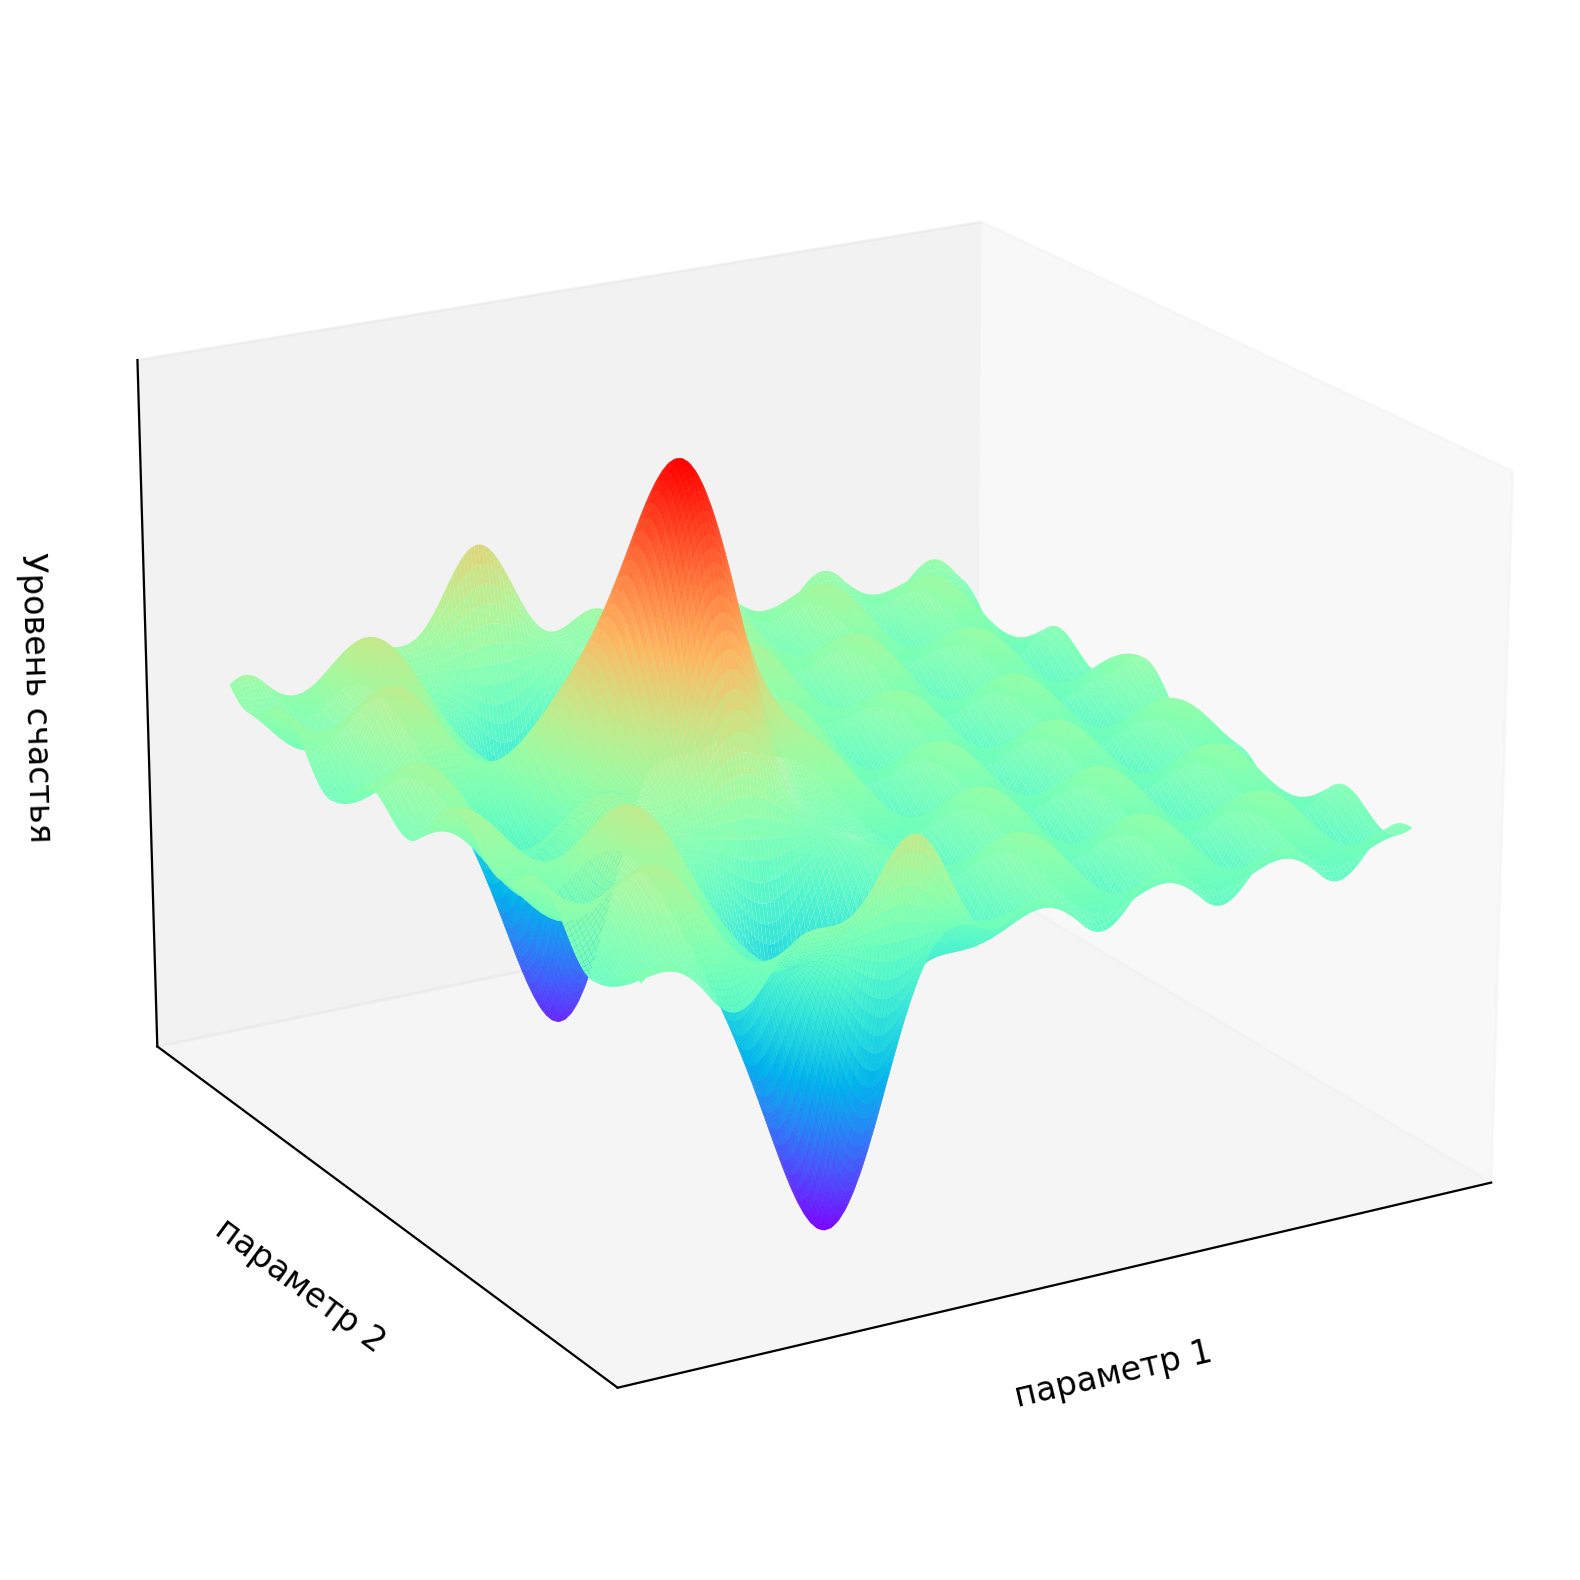
\includegraphics[width = \textwidth]{happines.png}  
        \column{0.5\textwidth}
        \begin{itemize}
            \item Нахождение глобальных минимумов/максимумов функции
            \item Нахождниие всех экстремумов
        \end{itemize}
    \end{columns}       
\end{frame}

\begin{frame}
    \frametitle{Минимизируемые функции}
    \begin{center}
        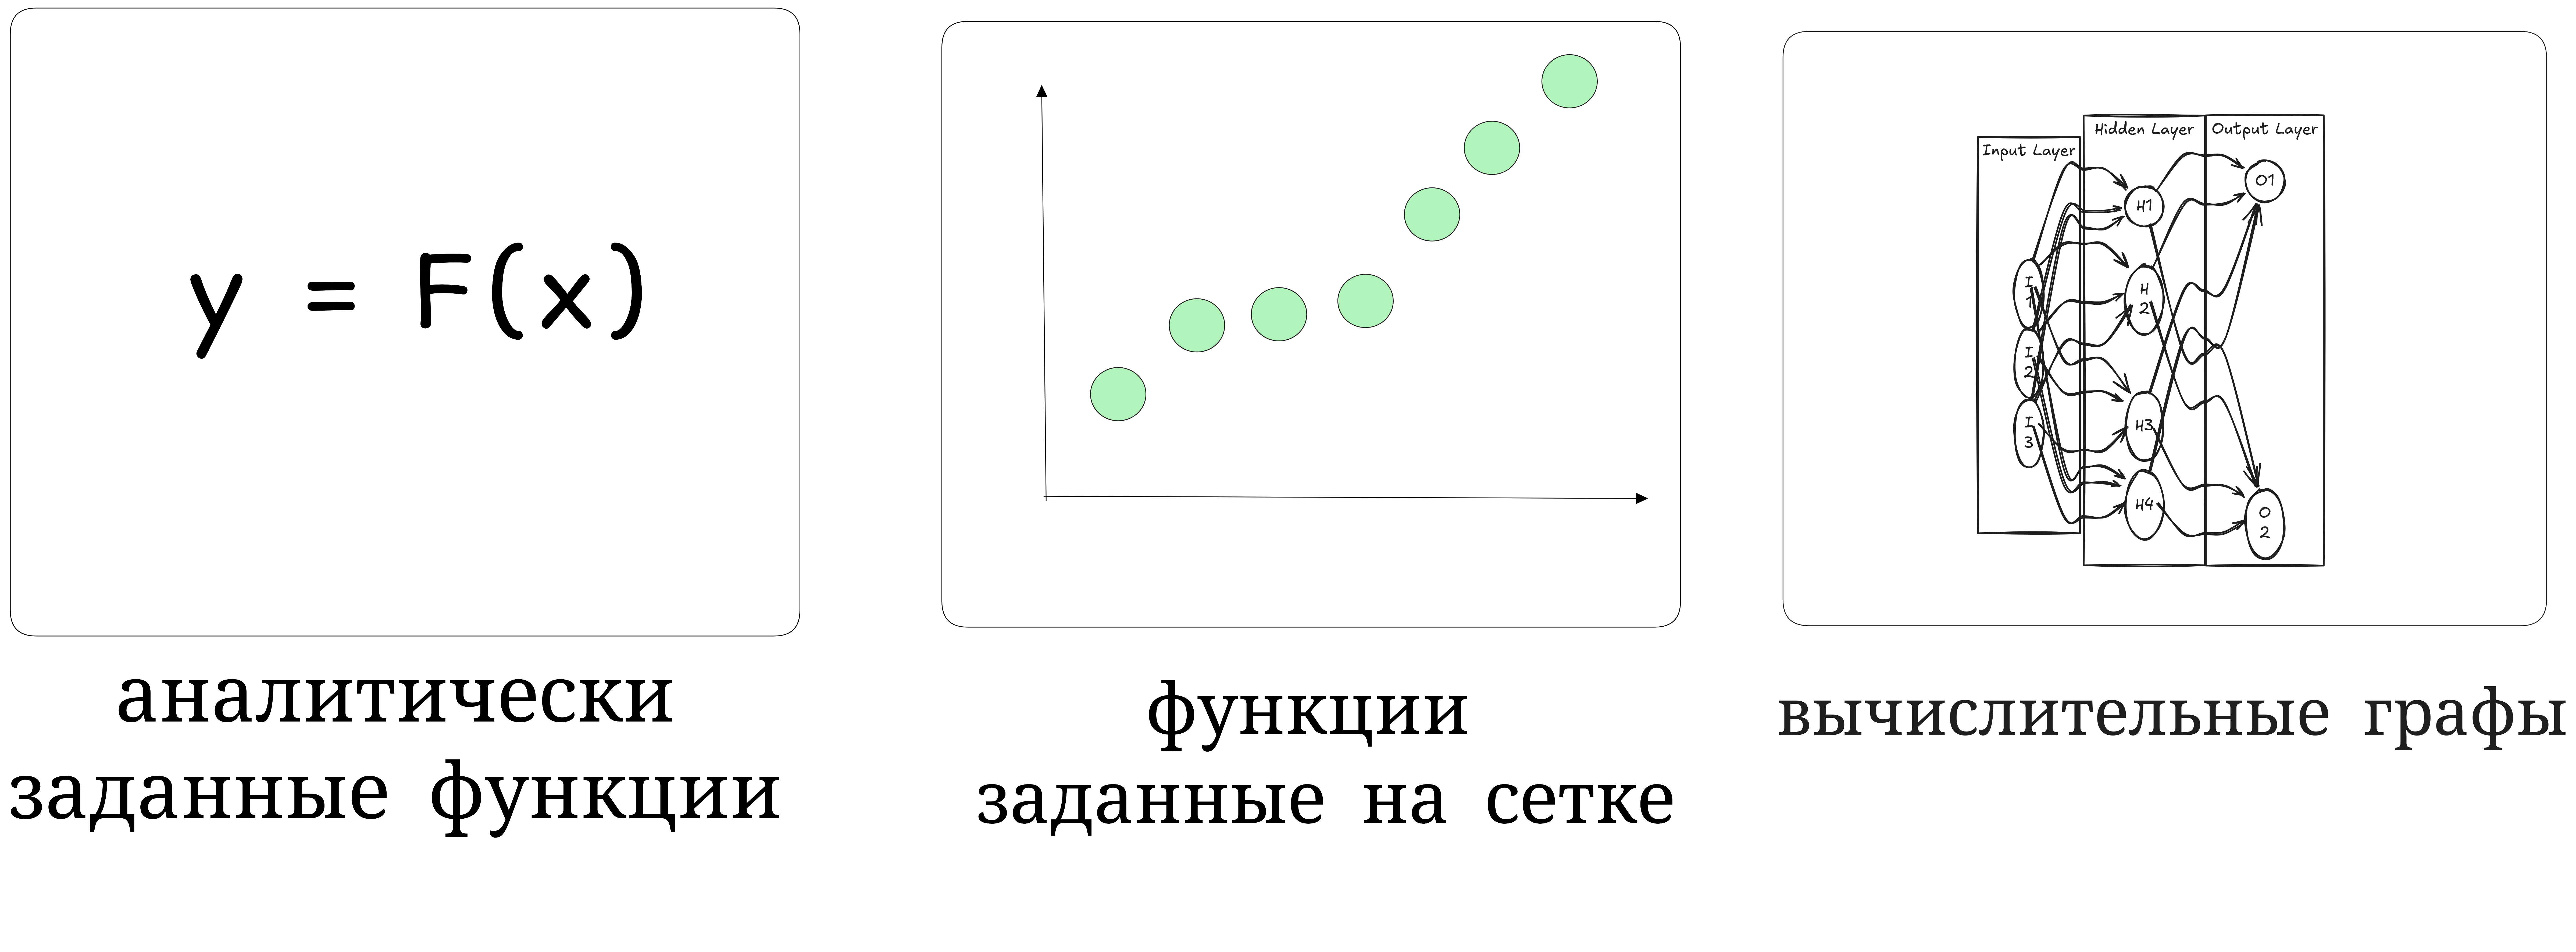
\includegraphics[width = 1\textwidth]{types.png}    
    \end{center}
    
\end{frame}

\begin{frame}
    \frametitle{Метод Фиббоначи}
    \begin{columns}
        
        \column{0.6\textwidth}
            \begin{enumerate}
            \item Задаём начальные границы a и b. 
            \item Пока количество итераций не превысило $N$:
            \begin{itemize}
                \item  Рассчитаем значения 
                $$
                    x_1 = a + (b - a) \frac{F_{n - 2}}{F_{n}}
                $$
                $$
                  x_2 = a + (b - a) \frac{F_{n - 1}}{F_{n}}
                $$
                \item Если $f(x_1) > f(x_2)$, то сужаем левую границу $a = x_1$.
                \item Иначе сужаем правую границу $b = x_2$.
            \end{itemize}
            \item Результат $(x_1 + x_2) / 2$
            
        \end{enumerate}   
    \end{columns} 
\end{frame}

\begin{frame}
    \frametitle{Метод Фиббоначи}
    \begin{center}
        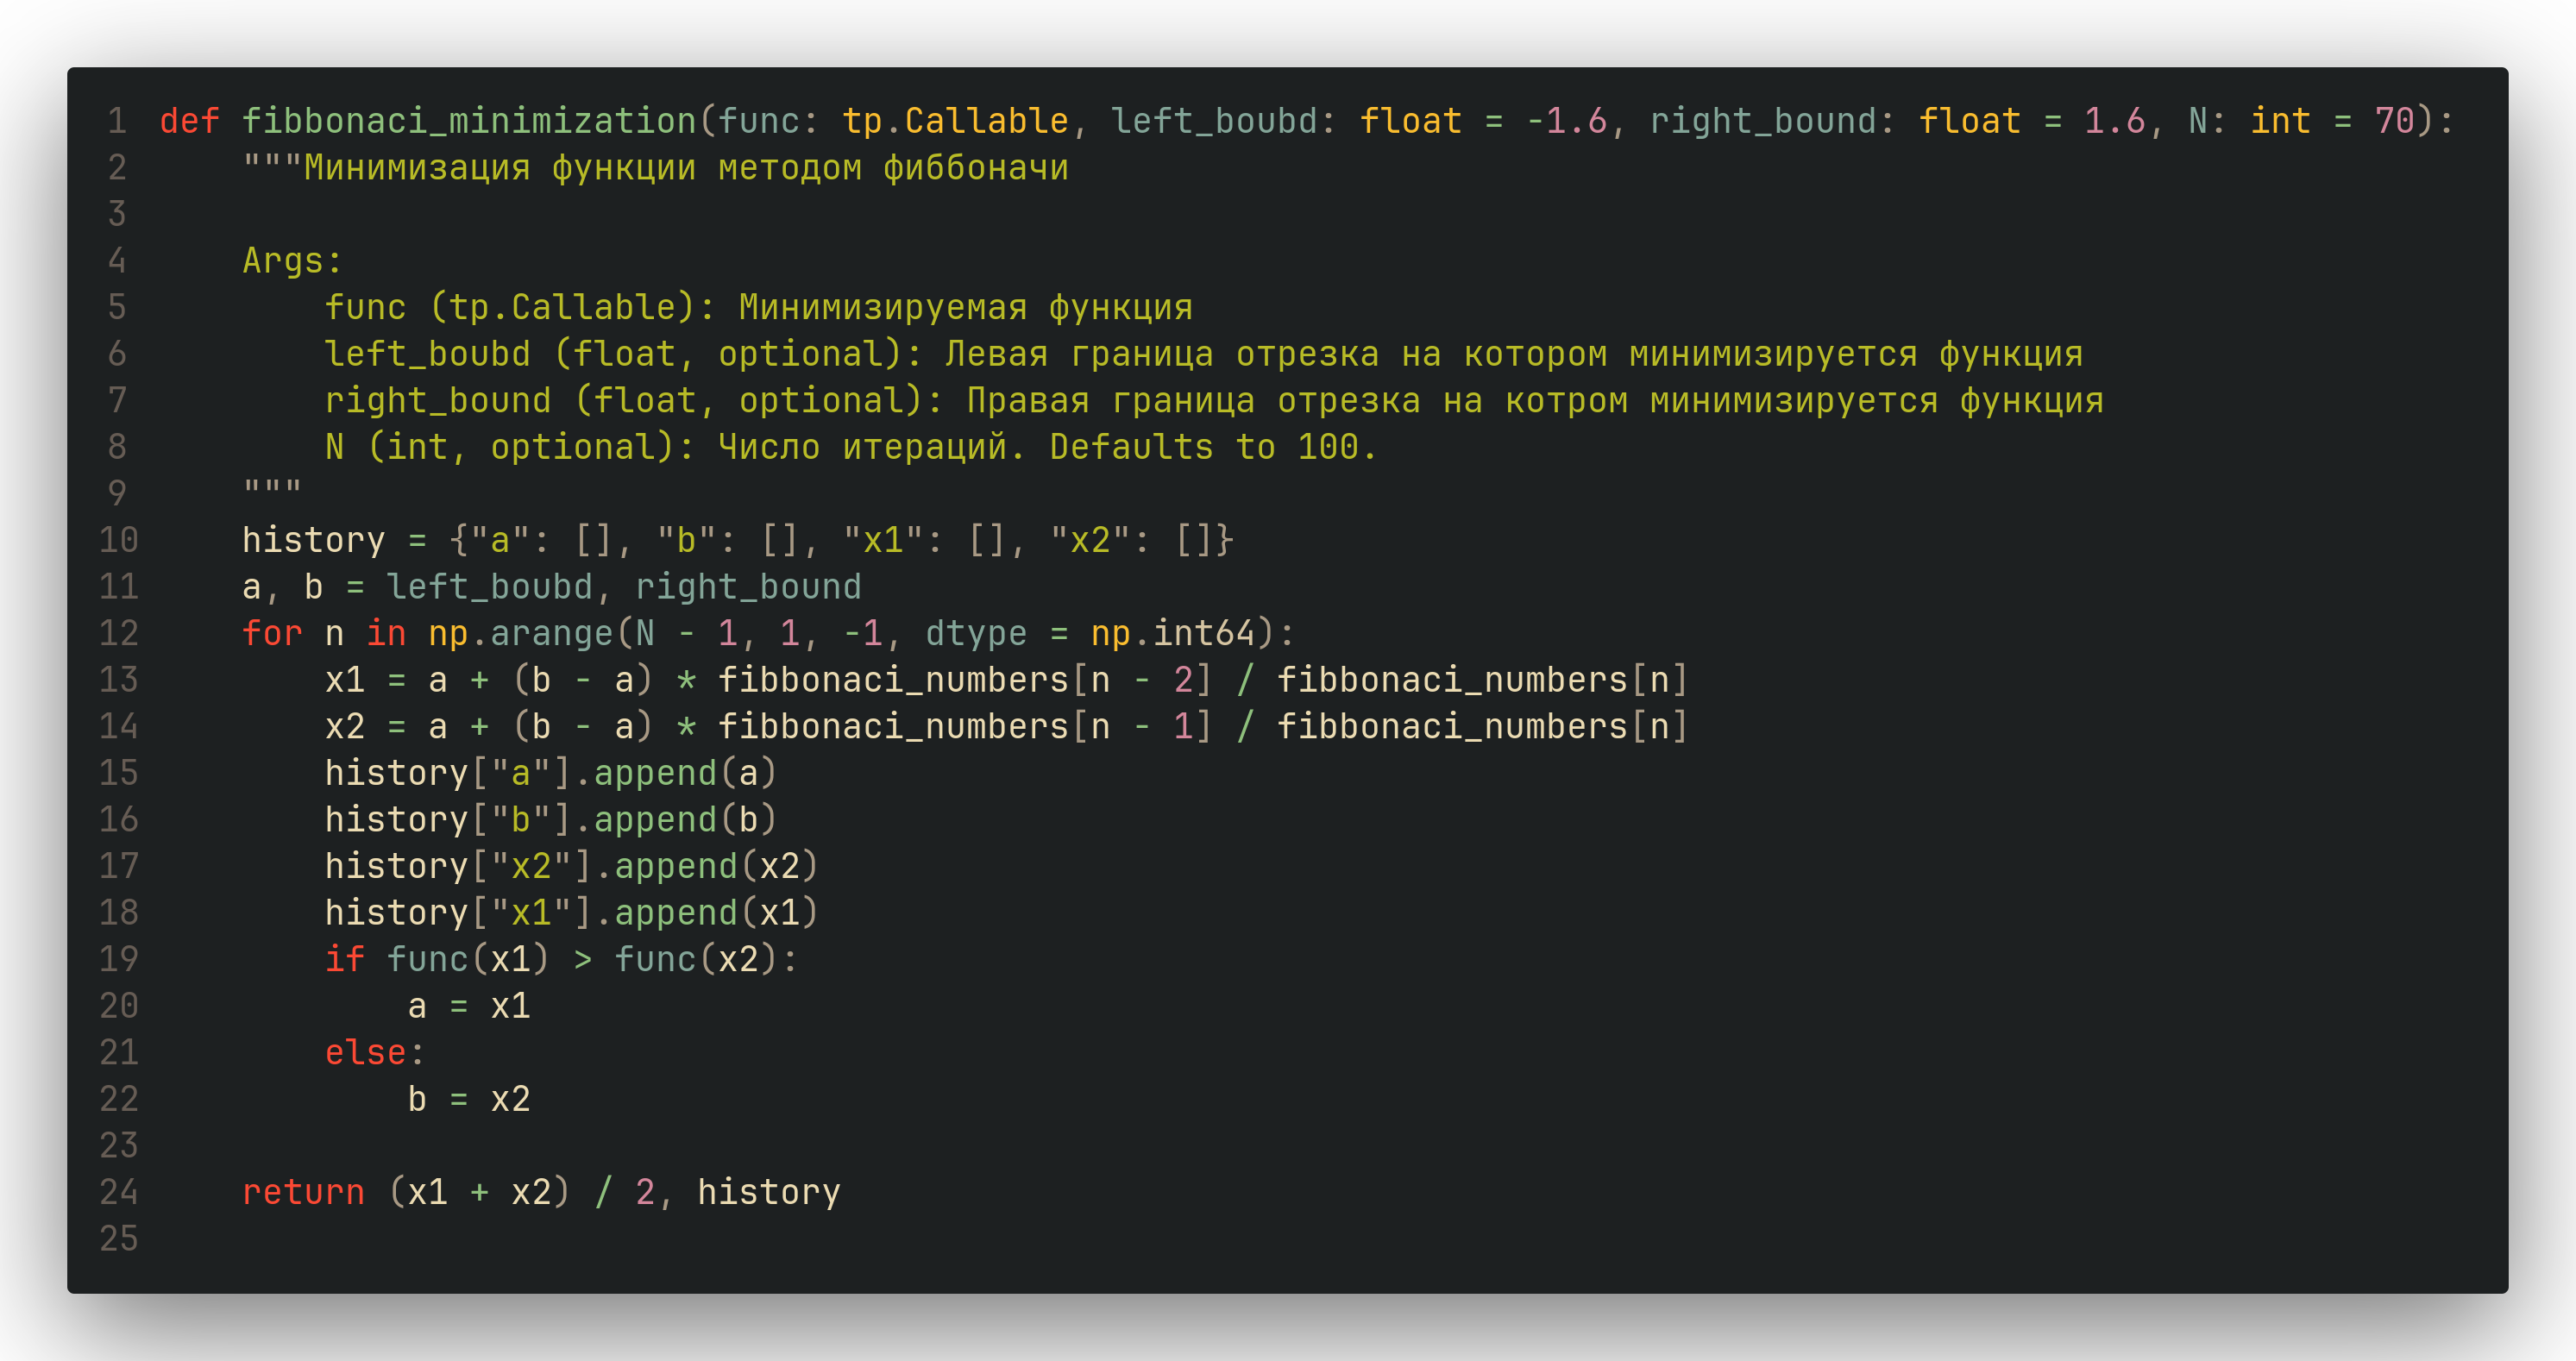
\includegraphics[width = 1\textwidth]{code_fibb.png}    
    \end{center}
    
\end{frame}



\begin{frame}
    \frametitle{Градиентный спуск}
    \begin{columns}
    
        \column{0.4\textwidth}
        \begin{enumerate}
            \item{Выбираем начальную точку $x_0$}
            \item{Пока не выполнено условие остановки}
            \begin{itemize}
                \item Вычсиляем $\nabla f(x_{k + 1})$
                \item Шаг градиентного спуска 
             
            \end{itemize}
        \end{enumerate}
        \begin{fequation}
            x_{k + 1} = x_k - \alpha \nabla f(x_{k + 1})
        \end{fequation}
        
        Константу $\alpha$ называют величиной шага(\textbf{step size}) или скоростью обучения (\textbf{learning rate})
        \column{0.6\textwidth}
        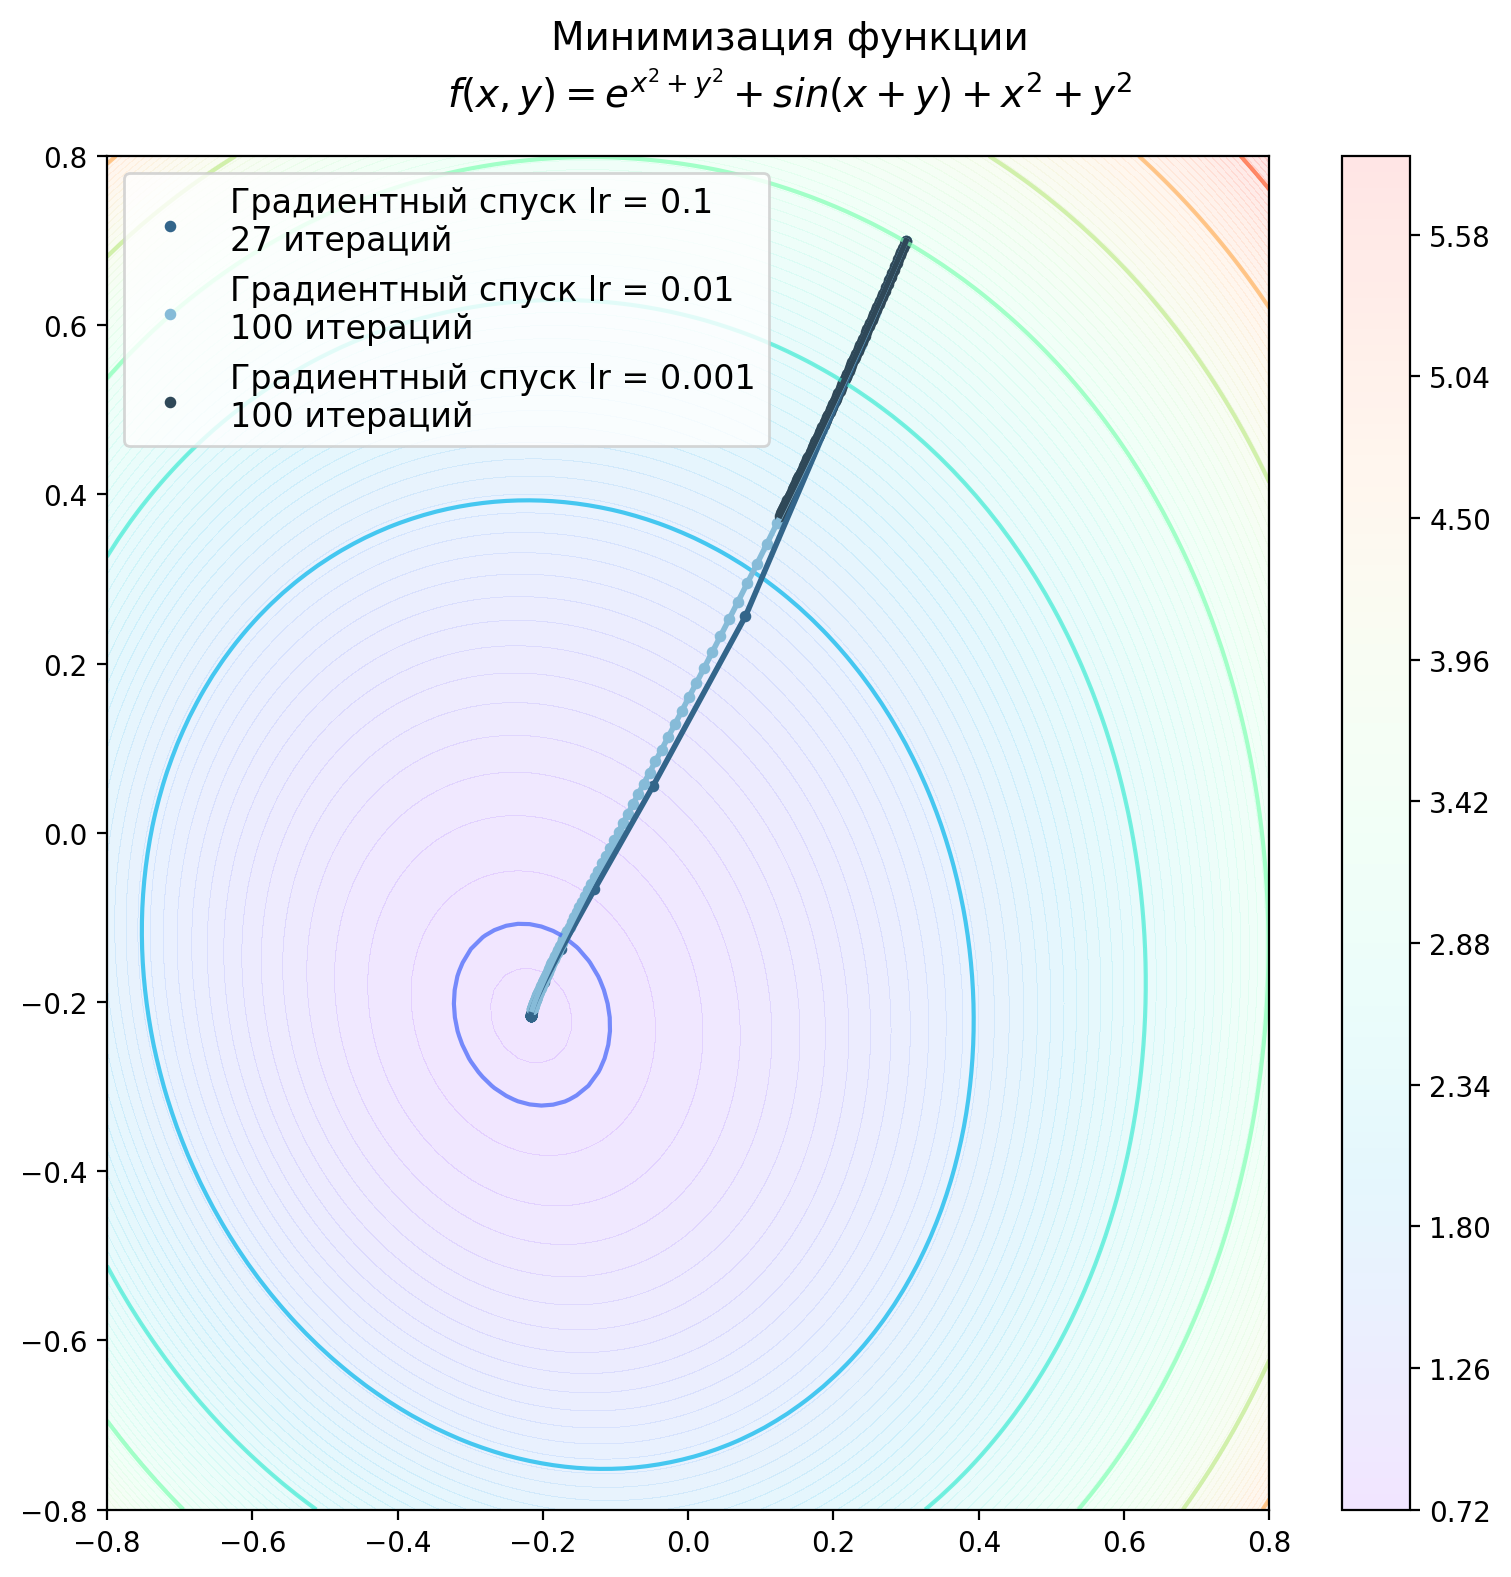
\includegraphics[width = 1\textwidth]{sgd.png}
    \end{columns}
\end{frame}

\begin{frame}
    \frametitle{Градиентный спуск}
    \begin{center}
        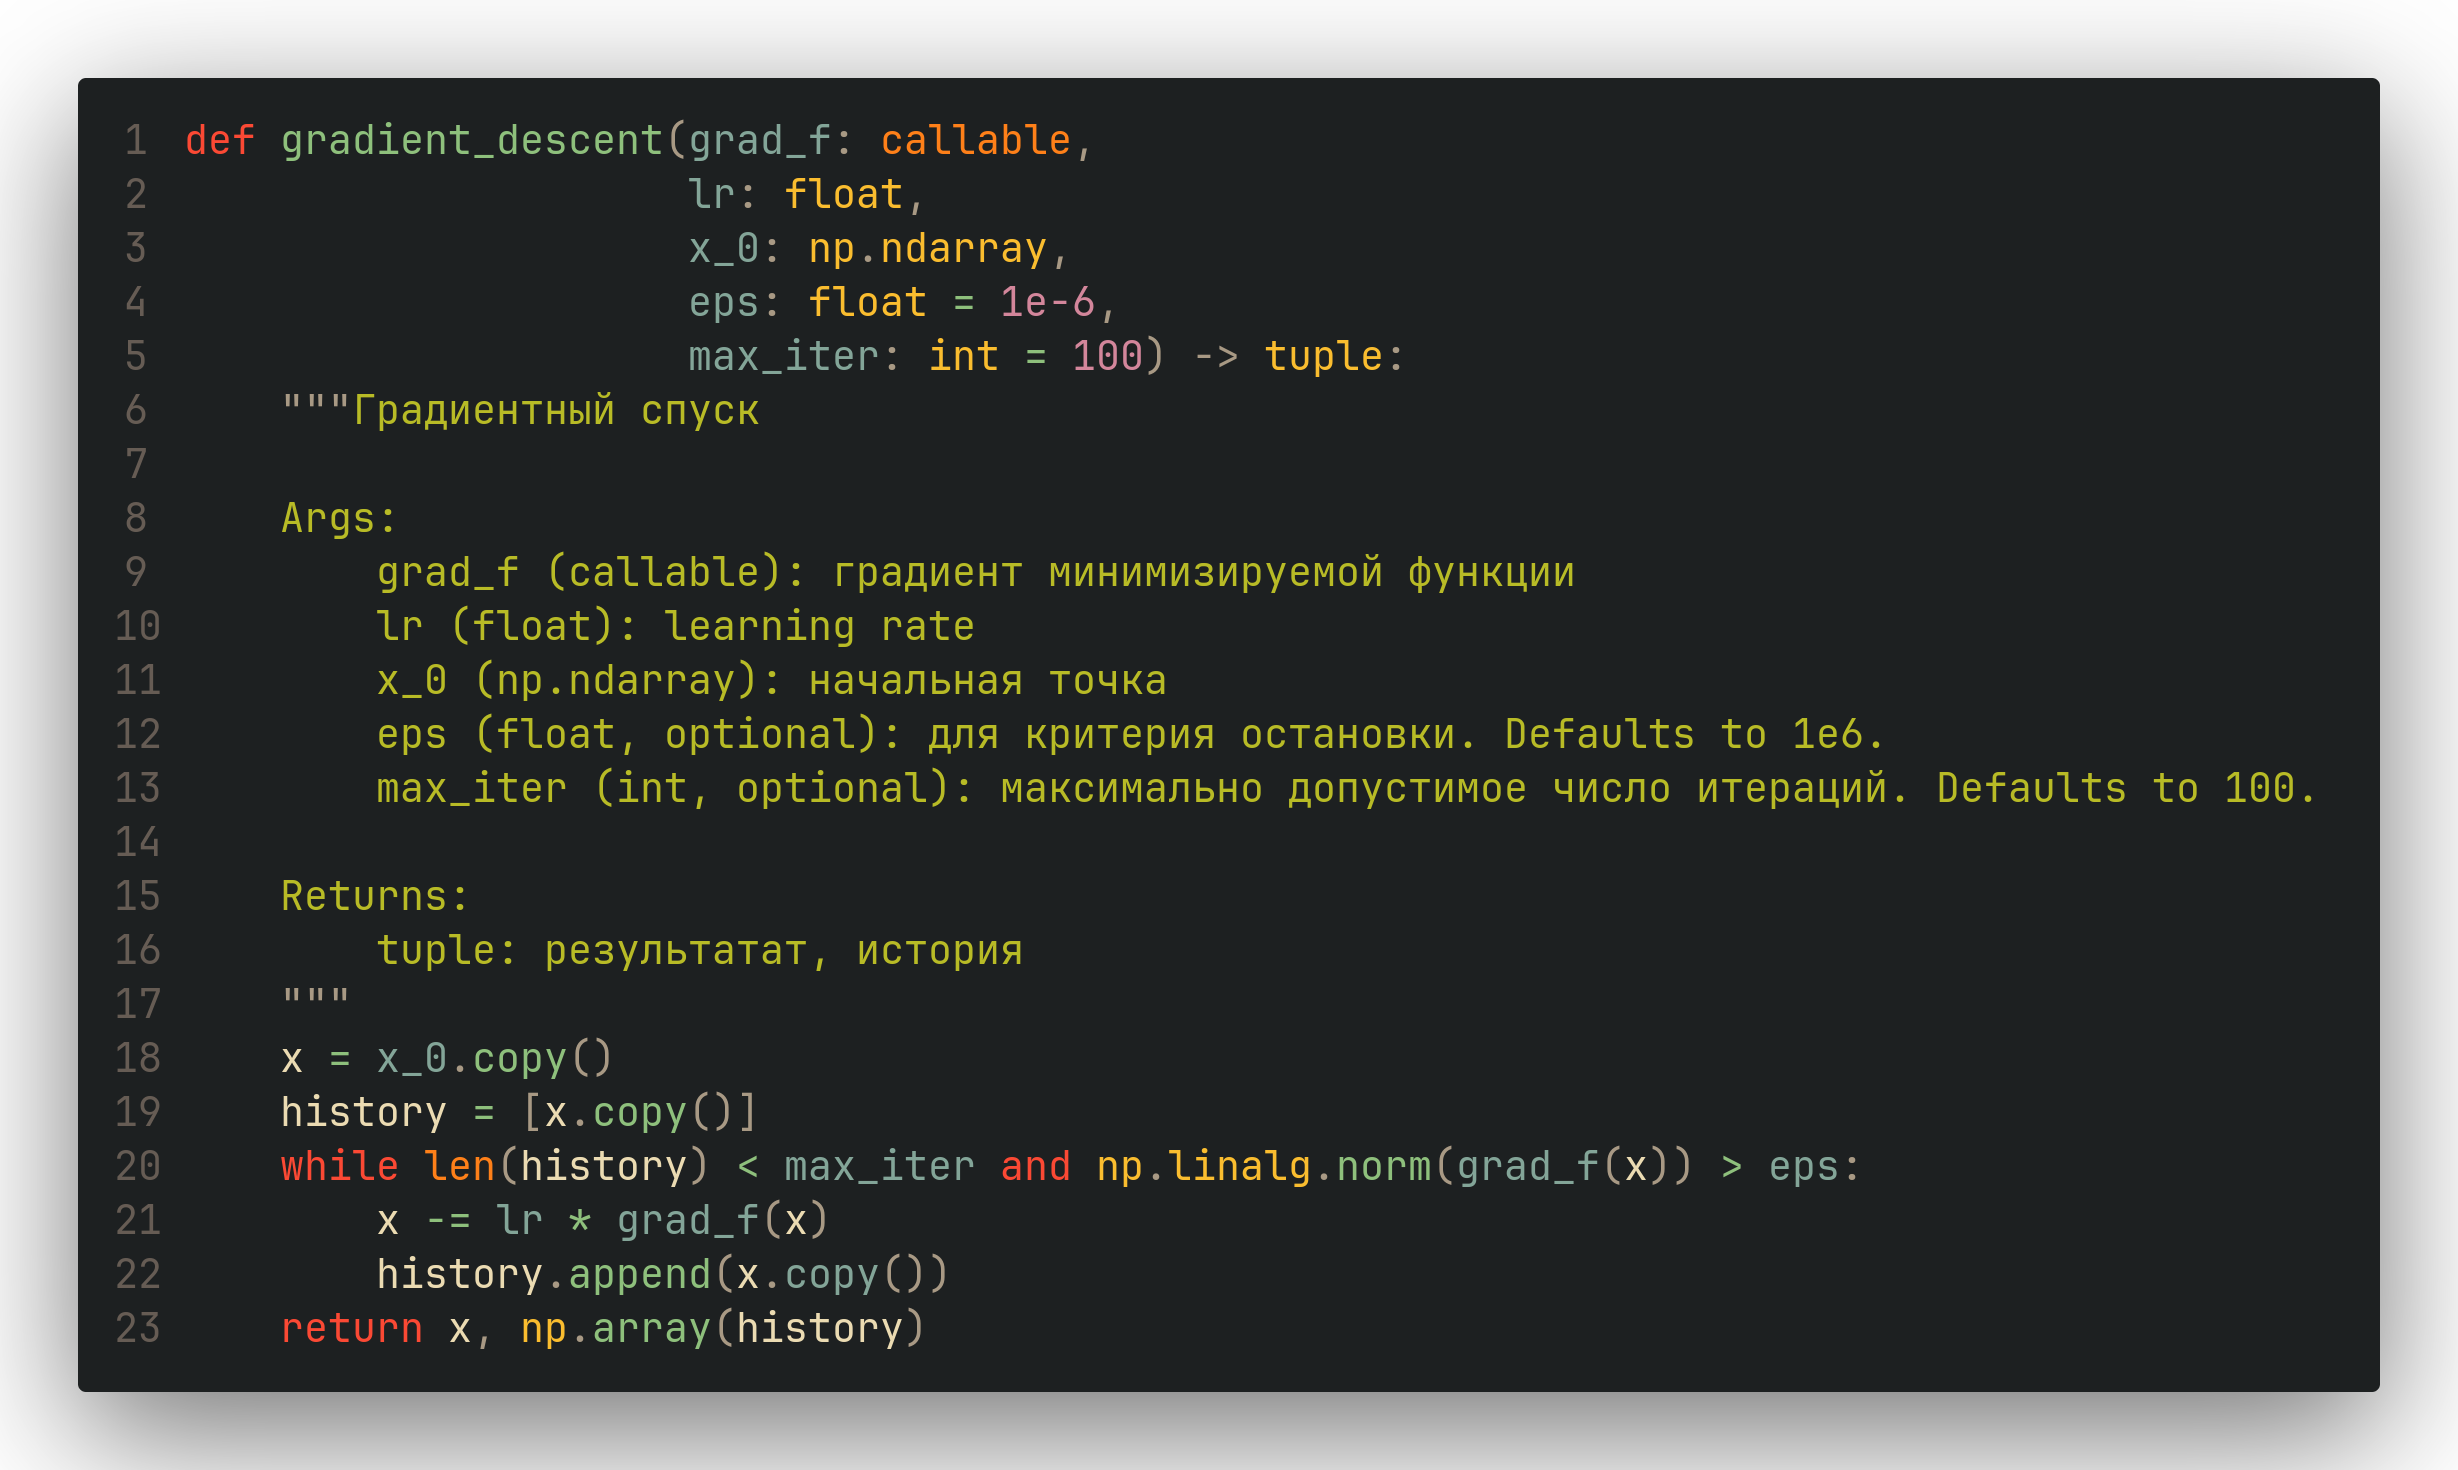
\includegraphics[width = 1\textwidth]{code_sgd.png}    
    \end{center}
    
\end{frame}


\begin{frame}
    \frametitle{Метод Ньютона}
    
\begin{columns}
    \column{0.5\textwidth}
    Пусть $f(x) \in C^{2}$. Выберем начальную точку $x_0$.Вместо функции $f$ рассмотрим её квадратичное приближение $F(x)$ в окрестности $x_0$:
    
   
    \column{0.5\textwidth}
    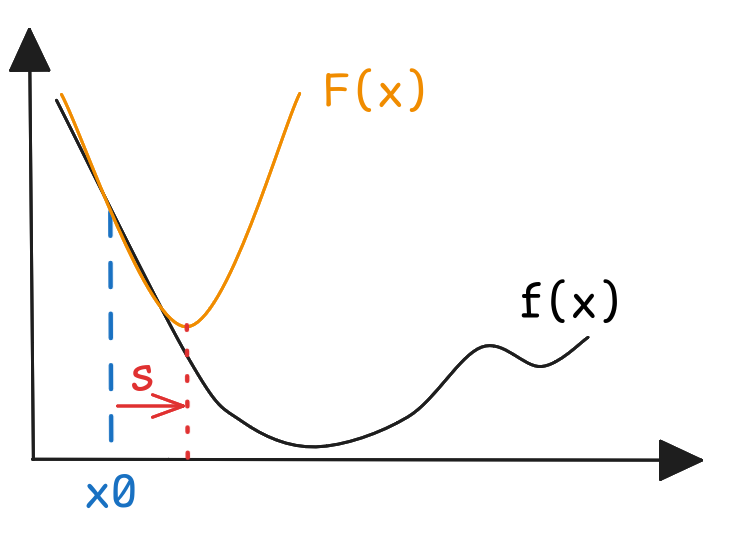
\includegraphics[width = 1\textwidth]{newton_expl.png}

    
\end{columns}
$$
F(\vec{x}) = f(\vec{x_0}) + \nabla f(\vec{x_0}) \cdot (\vec{x} - \vec{x_0}) + \frac{1}{2}(\vec{x} - \vec{x_0})^{T} G_{f}(\vec{x_0}) (\vec{x} - \vec{x_0})
$$

$$
\vec{s} = \vec{x} - \vec{x_0}
$$
$$
F(\vec{s}) = f(\vec{x_0}) + \nabla f(\vec{x_0}) \cdot \vec{s} + \frac{1}{2}\vec{s}^{T} G_{f}(\vec{x_0}) \vec{s}
$$
\end{frame}

\begin{frame}
    \frametitle{Метод Ньютона}
    \begin{center}
        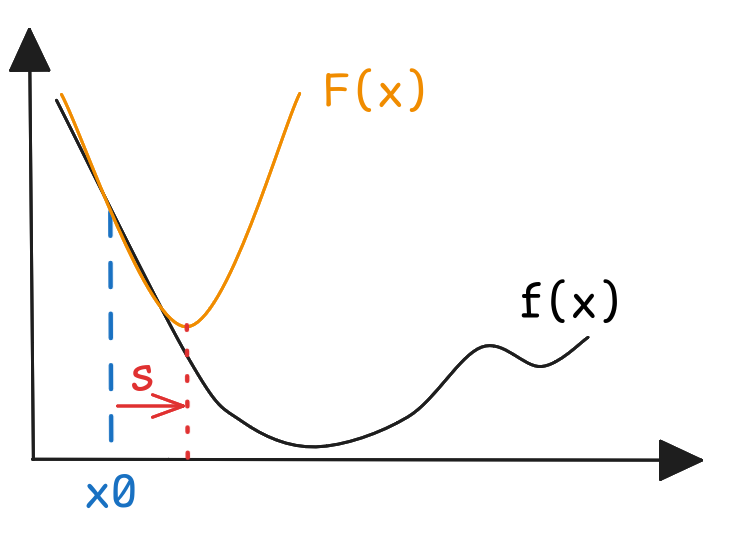
\includegraphics[width = 0.4\textwidth]{newton_expl.png}    
    \end{center}
    
    Найдём минимум функции $F$
    $$
    \nabla F(s) = 0 + \nabla f(\vec{x_0}) + \frac{1}{2} (G_{f}(\vec{x_0}) s + s^T G_{f}) = \nabla f(\vec{x_0}) + G_f s = 0
    $$

    $$
    s = -G_f^{-1}\nabla f(x_0) 
    $$

    \begin{fequation}
        x = x_0  - G_f^{-1}\nabla f(x_0)
    \end{fequation}

    Для использования метода Ньютона необходима \textbf{положительная определённость матрицы Гесса}.
     
    
\end{frame}


\begin{frame}
    \frametitle{Метод Ньютона}
    \begin{columns}
    
        \column{0.4\textwidth}
        \begin{enumerate}
            \item{Выбираем начальную точку $x_0$}
            \item{Пока не выполнено условие остановки}
            \begin{itemize}
                \item Вычсиляем $\nabla f(x_{k + 1})$ и $G_{f}^{-1}(x_k)$
                \item Шаг метода Ньютона
            \end{itemize}
        \end{enumerate}
        \begin{fequation}
            x_{k+1} = x_k - G_f^{-1}(x_k)\nabla f(x_0)
        \end{fequation}
        \column{0.6\textwidth}
        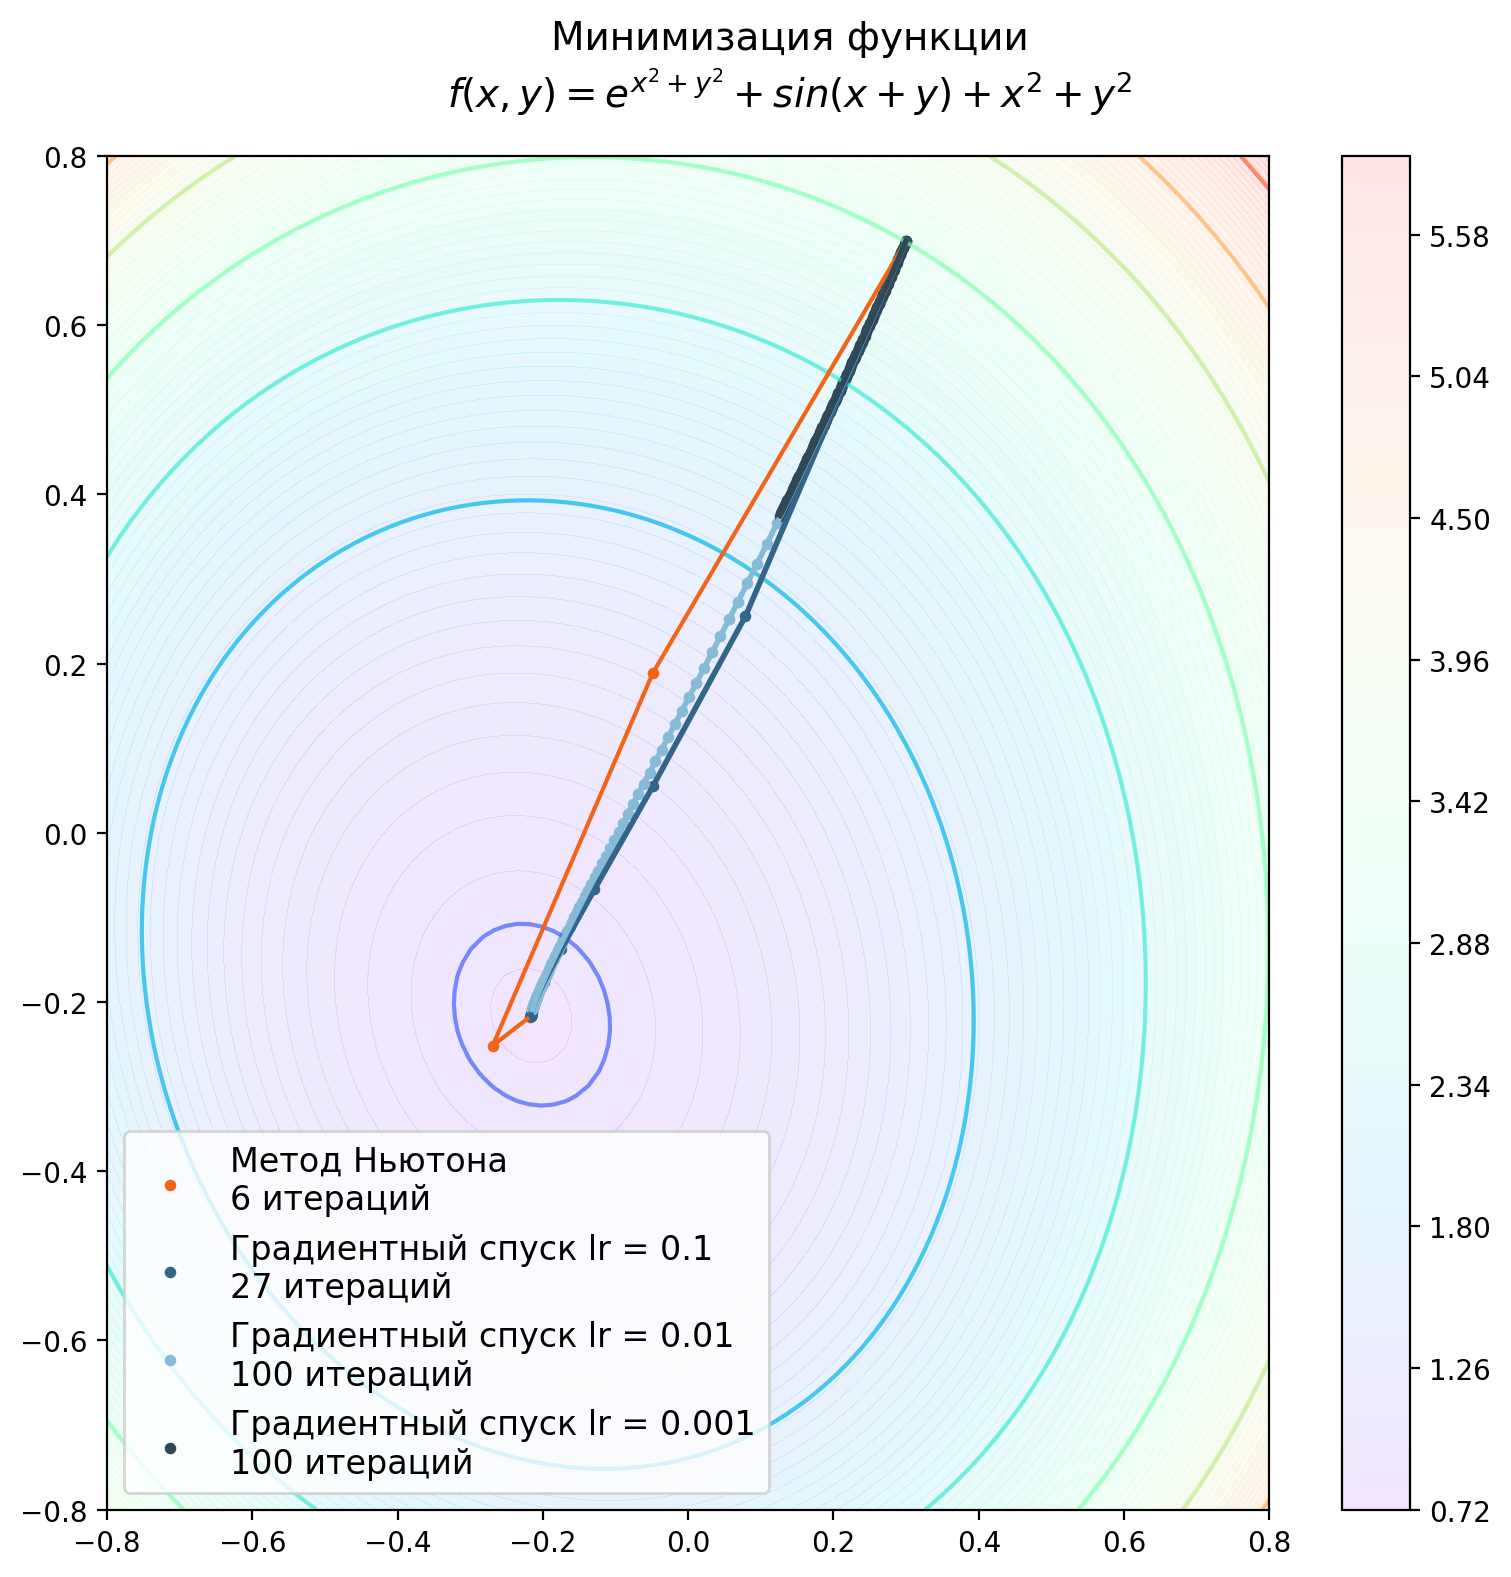
\includegraphics[width = 1\textwidth]{sgd_and_newton.png}
    \end{columns}
\end{frame}


\begin{frame}
    \frametitle{Метод Ньютона}
    \begin{center}
        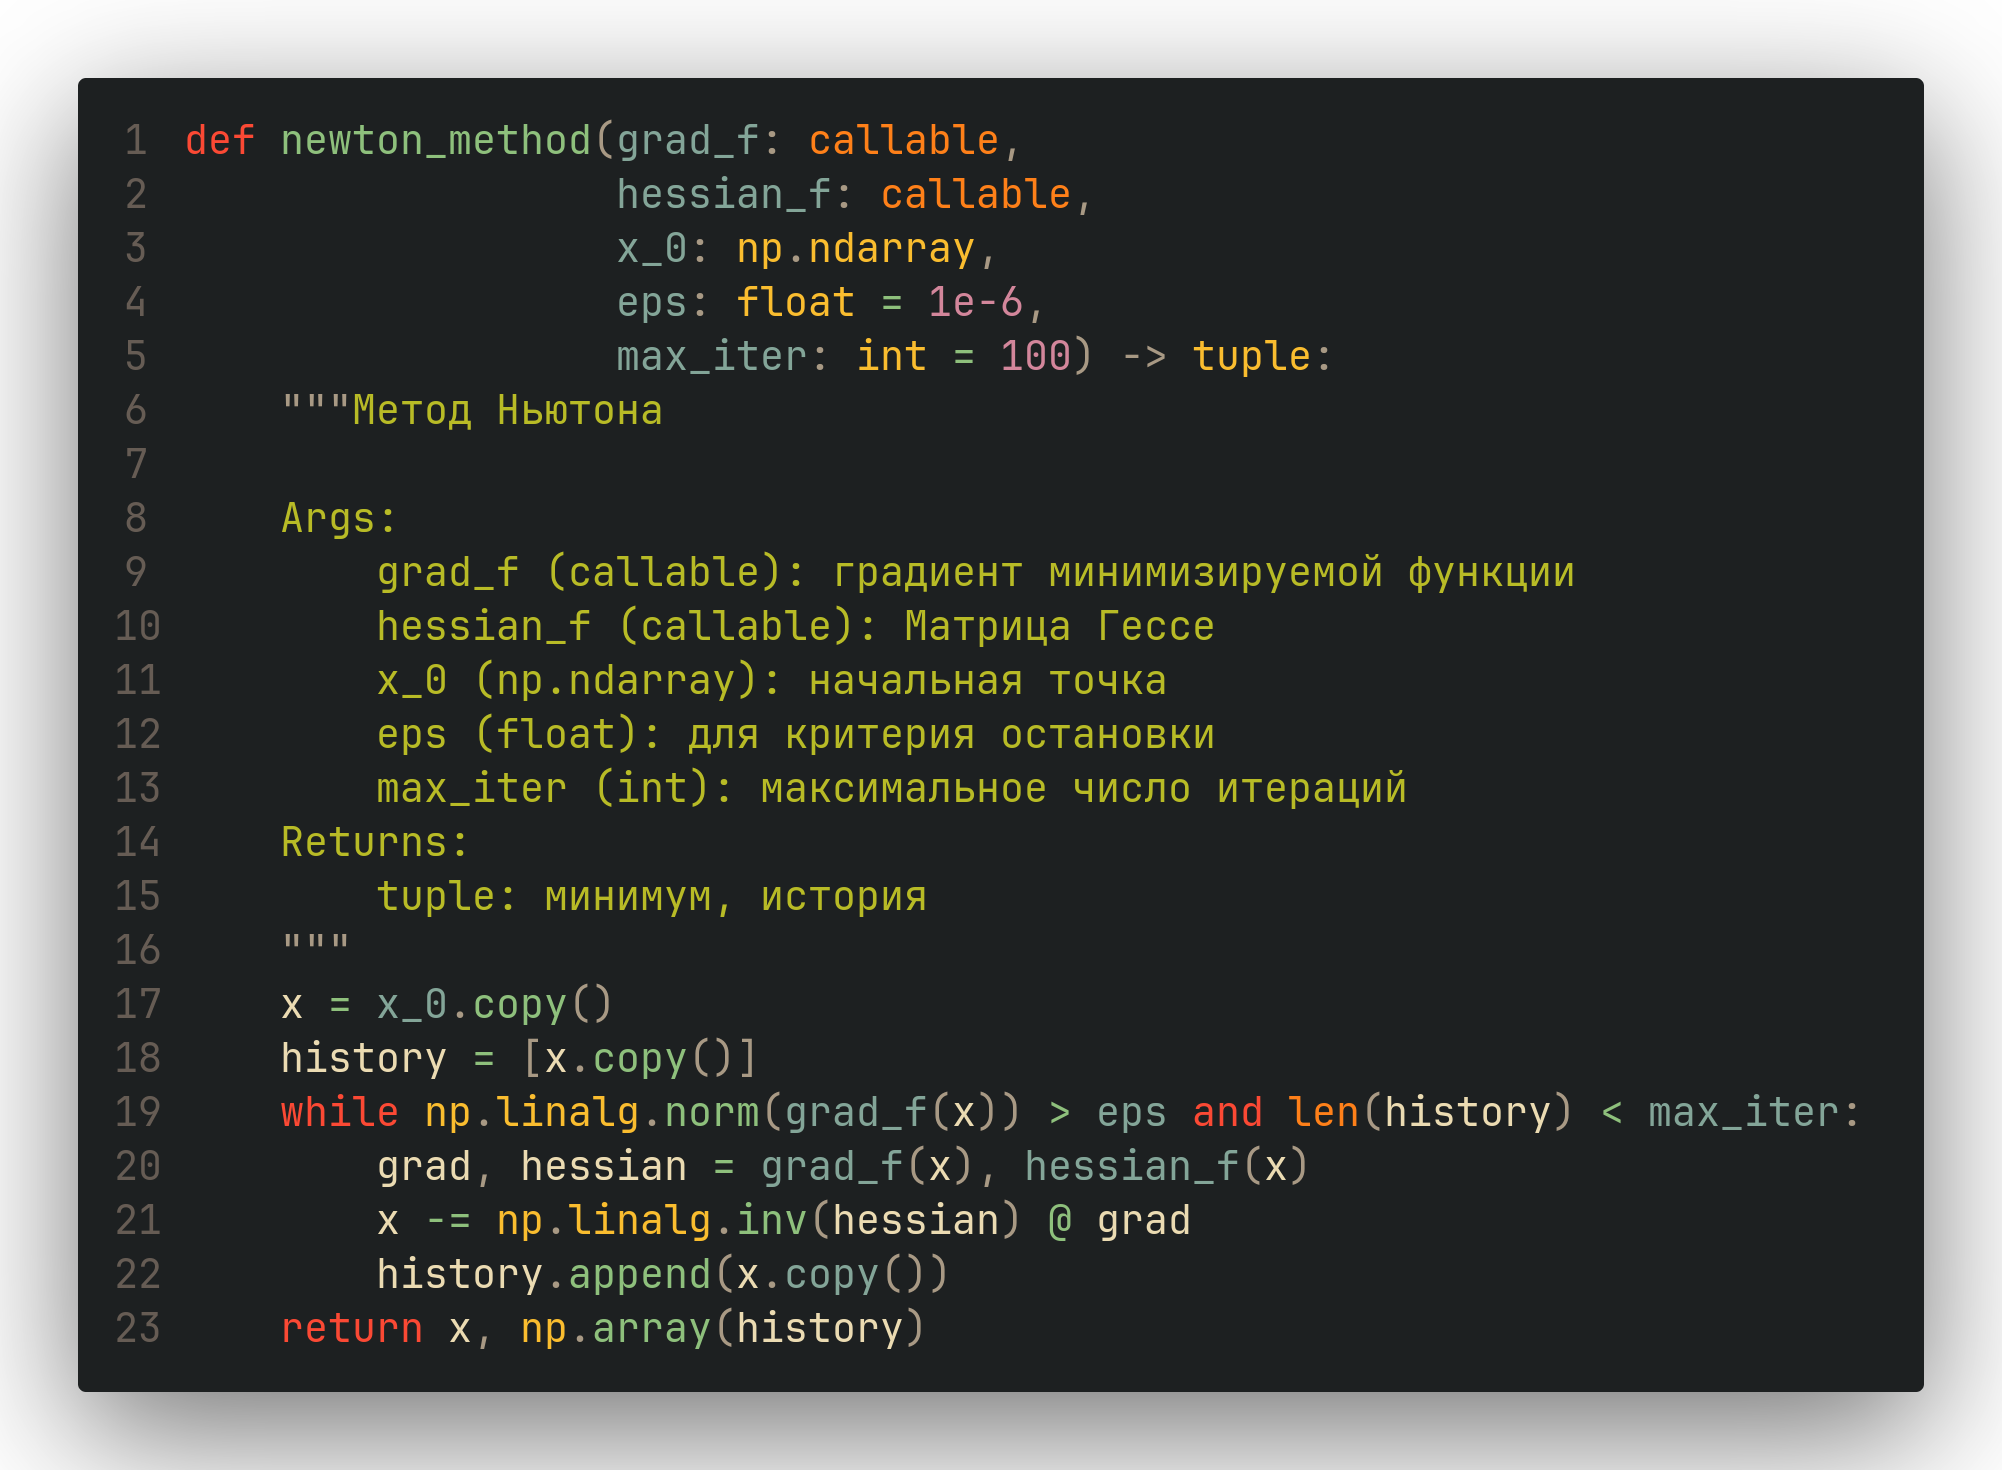
\includegraphics[width = 1\textwidth]{code_newton.png}
    \end{center}
\end{frame}


\begin{frame}
    \frametitle{Метод Ньютона}
    \begin{center}
        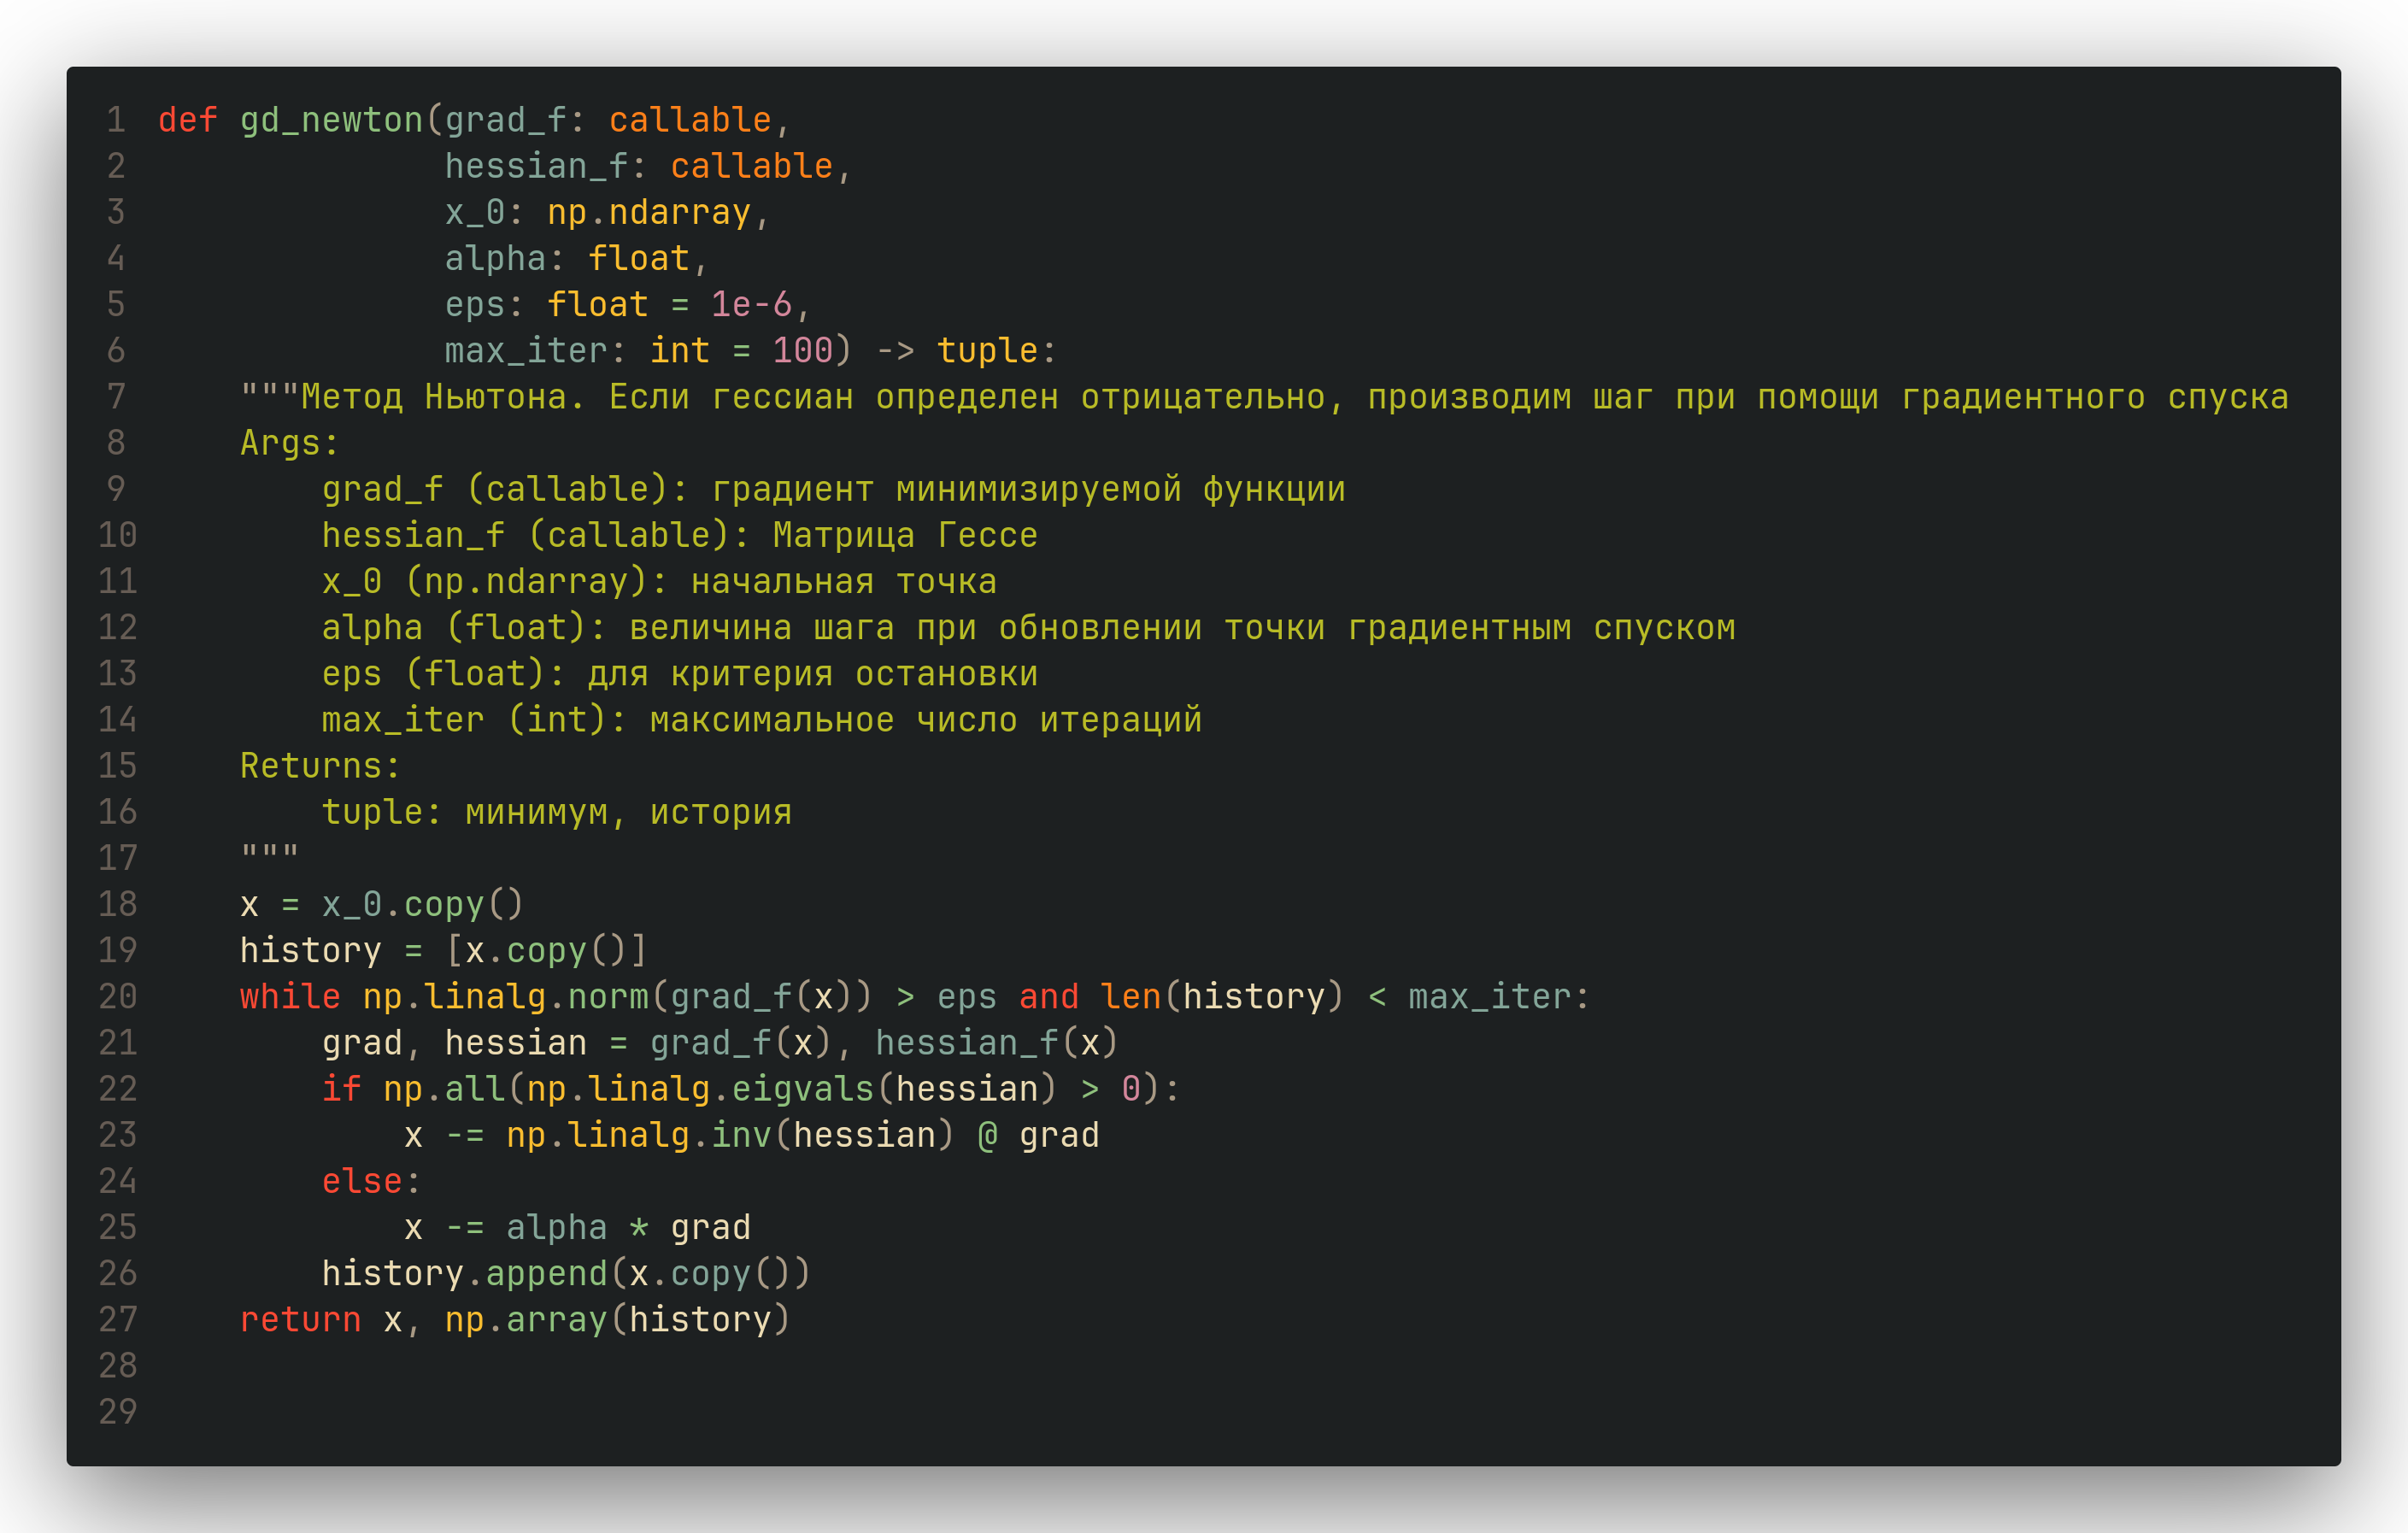
\includegraphics[width = 1\textwidth]{code_newton_2.png}
    \end{center}
\end{frame}

\begin{frame}
    \frametitle{Улучшение градиентного спуска}
    
    \begin{columns}
        \column{0.5\textwidth}
        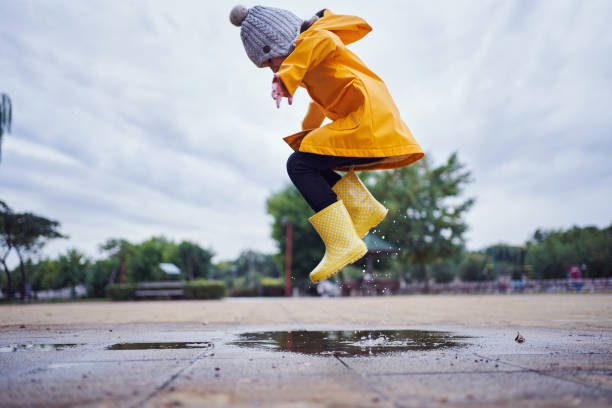
\includegraphics[width = 0.9\textwidth]{luzha.jpg}
        Изменять величину шага в зависимости от обстоятельств
        \column{0.5\textwidth}
        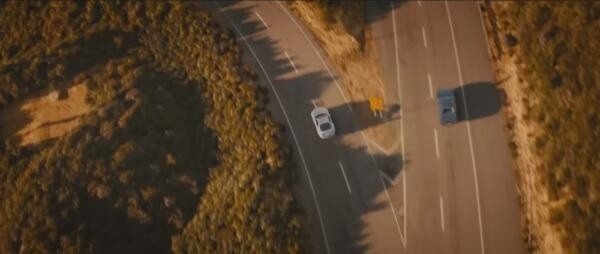
\includegraphics[width = 0.9\textwidth]{razvilka.jpg}
        При выборе нового направления учитывать предыдущее направление
    \end{columns}
\end{frame}


\begin{frame}
    \frametitle{Метод сопряженных градиентов}
    \begin{columns}
        \column{0.6\textwidth}
        \begin{enumerate}
            \item Выбрать начальную точку $x_0$. В качестве начального направления выберем направление антиградинета $S_{0} = -\nabla f(x_0)$.
            \item Пока не выполнено условие остановки
            \begin{itemize}
                \item Сконструируем функцию одной переменной $\phi(t) = f(x_k + t \cdot S_{k})$. 
                \item Найдём минимум функции $\phi$. $x_{k+1} = x_k + t_{opt} \cdot S_{k}$
                \item Вычислим новое направление 
                
                
            \end{itemize} 
        \end{enumerate}
        \begin{fequation}
            S_{k + 1} = \nabla f(x_{k + 1}) + \beta(\nabla f(x_{k+1}), \nabla f(x_{k}), S_{k}) S_{k}    
        \end{fequation}
        \column{0.4\textwidth}
        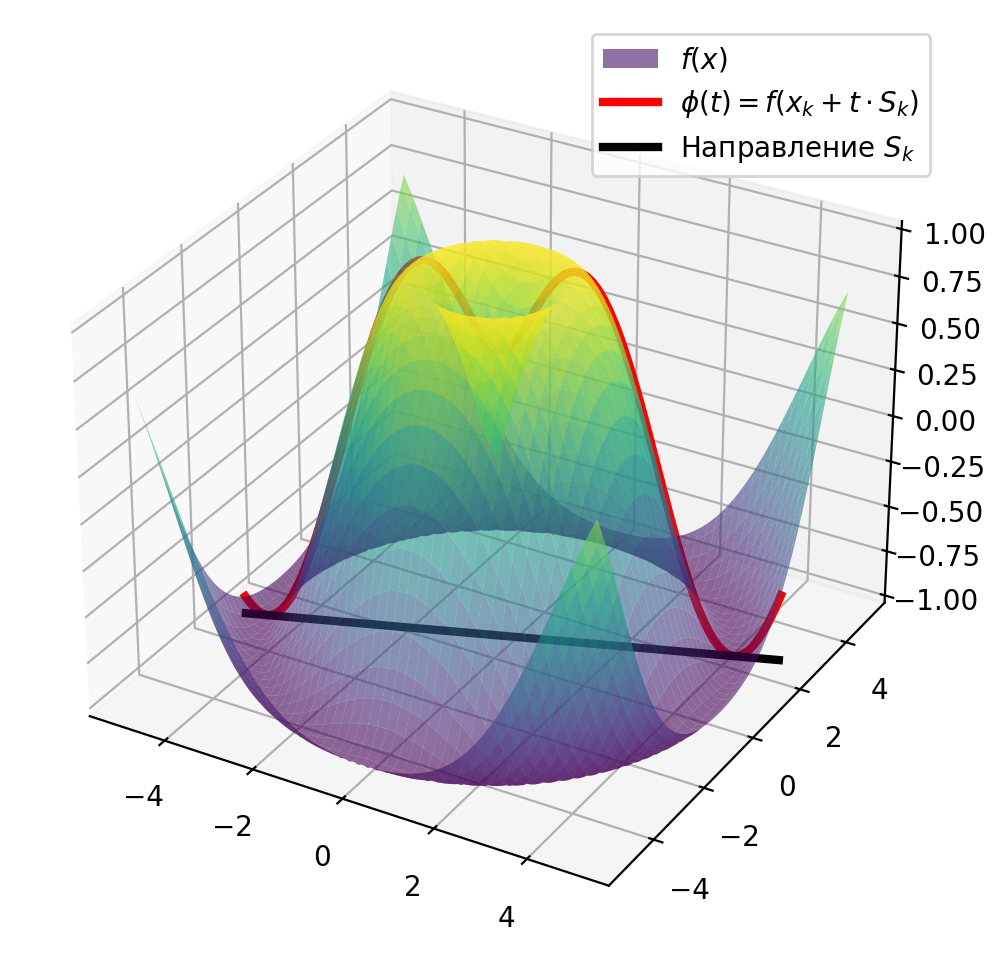
\includegraphics[width = 1\textwidth]{grad_expl_1.png}
    \end{columns}
\end{frame}

\begin{frame}
    \frametitle{Метод сопряженных градиентов}
    Метод сопряженных градиентов - класс методов, отличающихся функциями $\beta(\nabla f(x_{k+1}), \nabla f(x_{k}), S_{k})$
    \begin{itemize}
        \item $$\beta_k^{HS} = \frac{\langle \nabla f(x_{k + 1}), \nabla f(x_{k + 1}) - \nabla f(x_{k}) \rangle}{\langle S_k, \nabla f(x_{k + 1}) - \nabla f(x_{k}) \rangle} \quad \text{Хестенс, Штифель}$$
        \item $$\beta_k^{FR} = \frac{|\nabla f(x_{k + 1})|^2}{|\nabla f(x_{k})|^2} \quad \text{Флетчер, Ривз}$$
        \item $$\beta_k^{PR} = \frac{\langle \nabla f(x_{k + 1}), \nabla f(x_{k + 1}) - \nabla f(x_{k}) \rangle}{|\nabla f(x_{k + 1})|^2} \quad \text{Полак, Рибьер }$$
        \item \dots
    \end{itemize}
\end{frame}

\begin{frame}
    \frametitle{Метод сопряженных градиентов}
    \begin{center}
        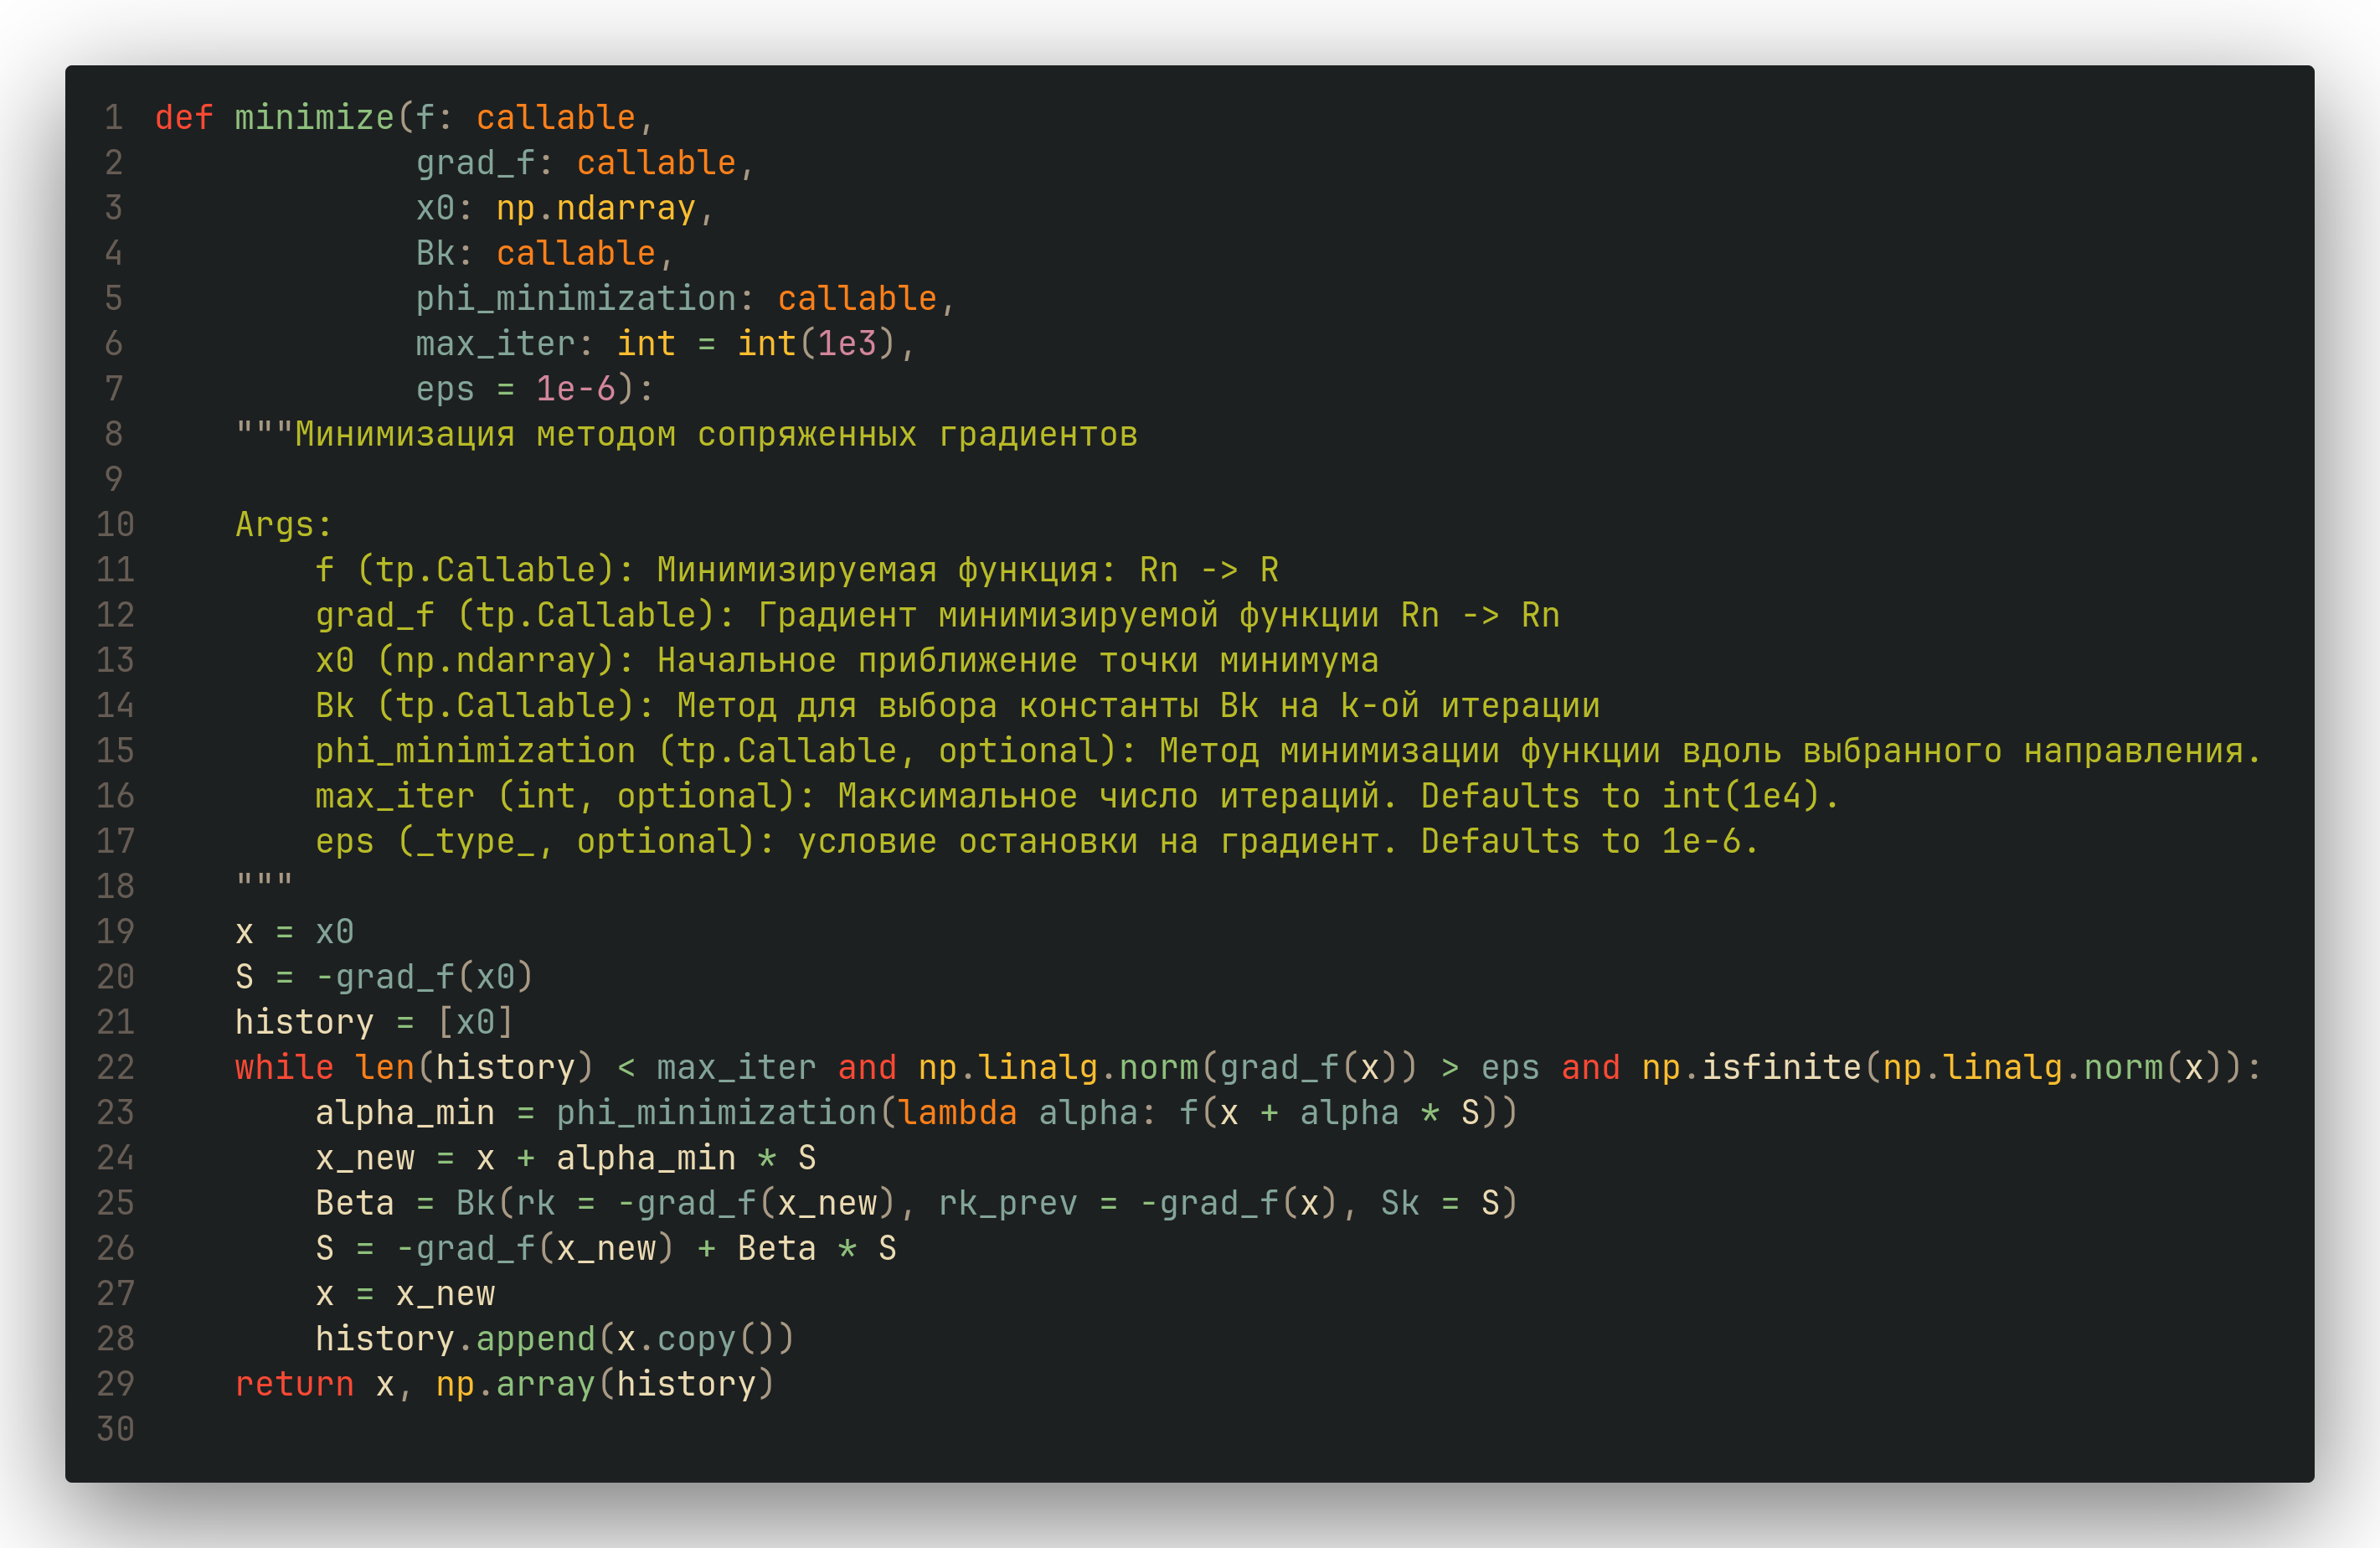
\includegraphics[width=1\textwidth]{code_gradient.png}    
    \end{center}
\end{frame}

\begin{frame}
    \frametitle{Метод сопряженных градиентов}
    \begin{center}
        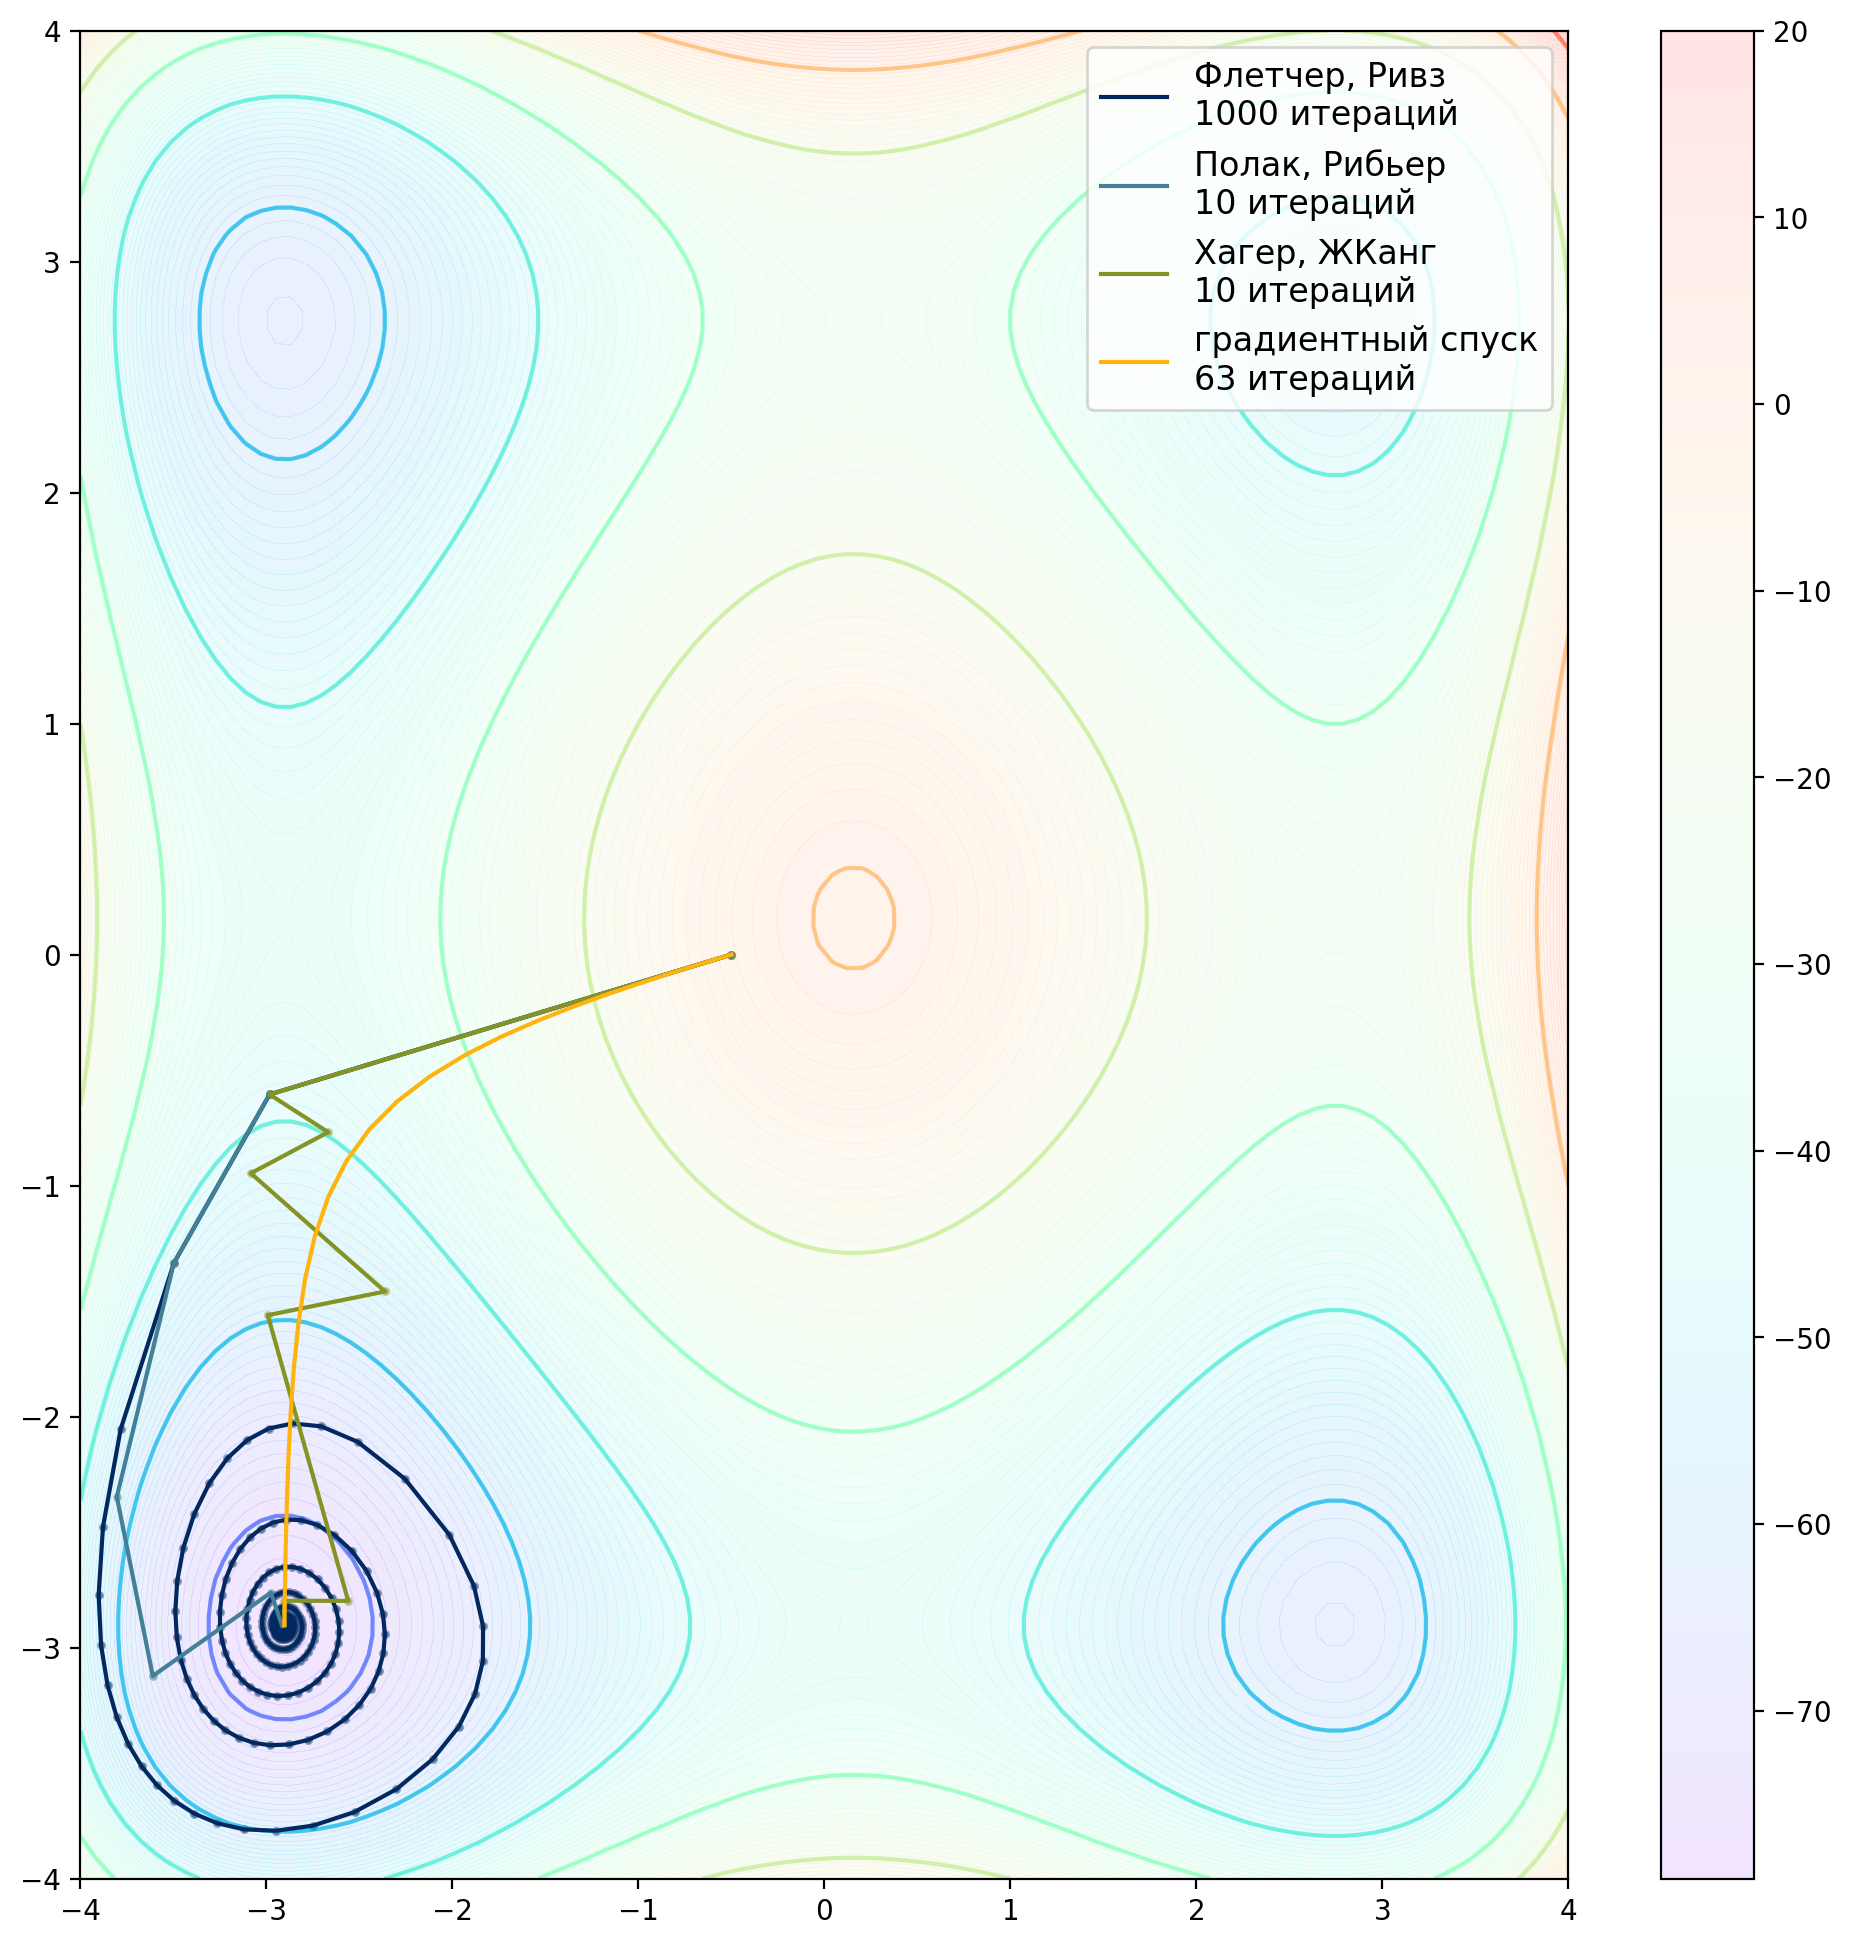
\includegraphics[width=0.7\textwidth]{grad_1.png}    
    \end{center}
\end{frame}


\begin{frame}
    \frametitle{Метод сопряженных градиентов}
    \begin{center}
        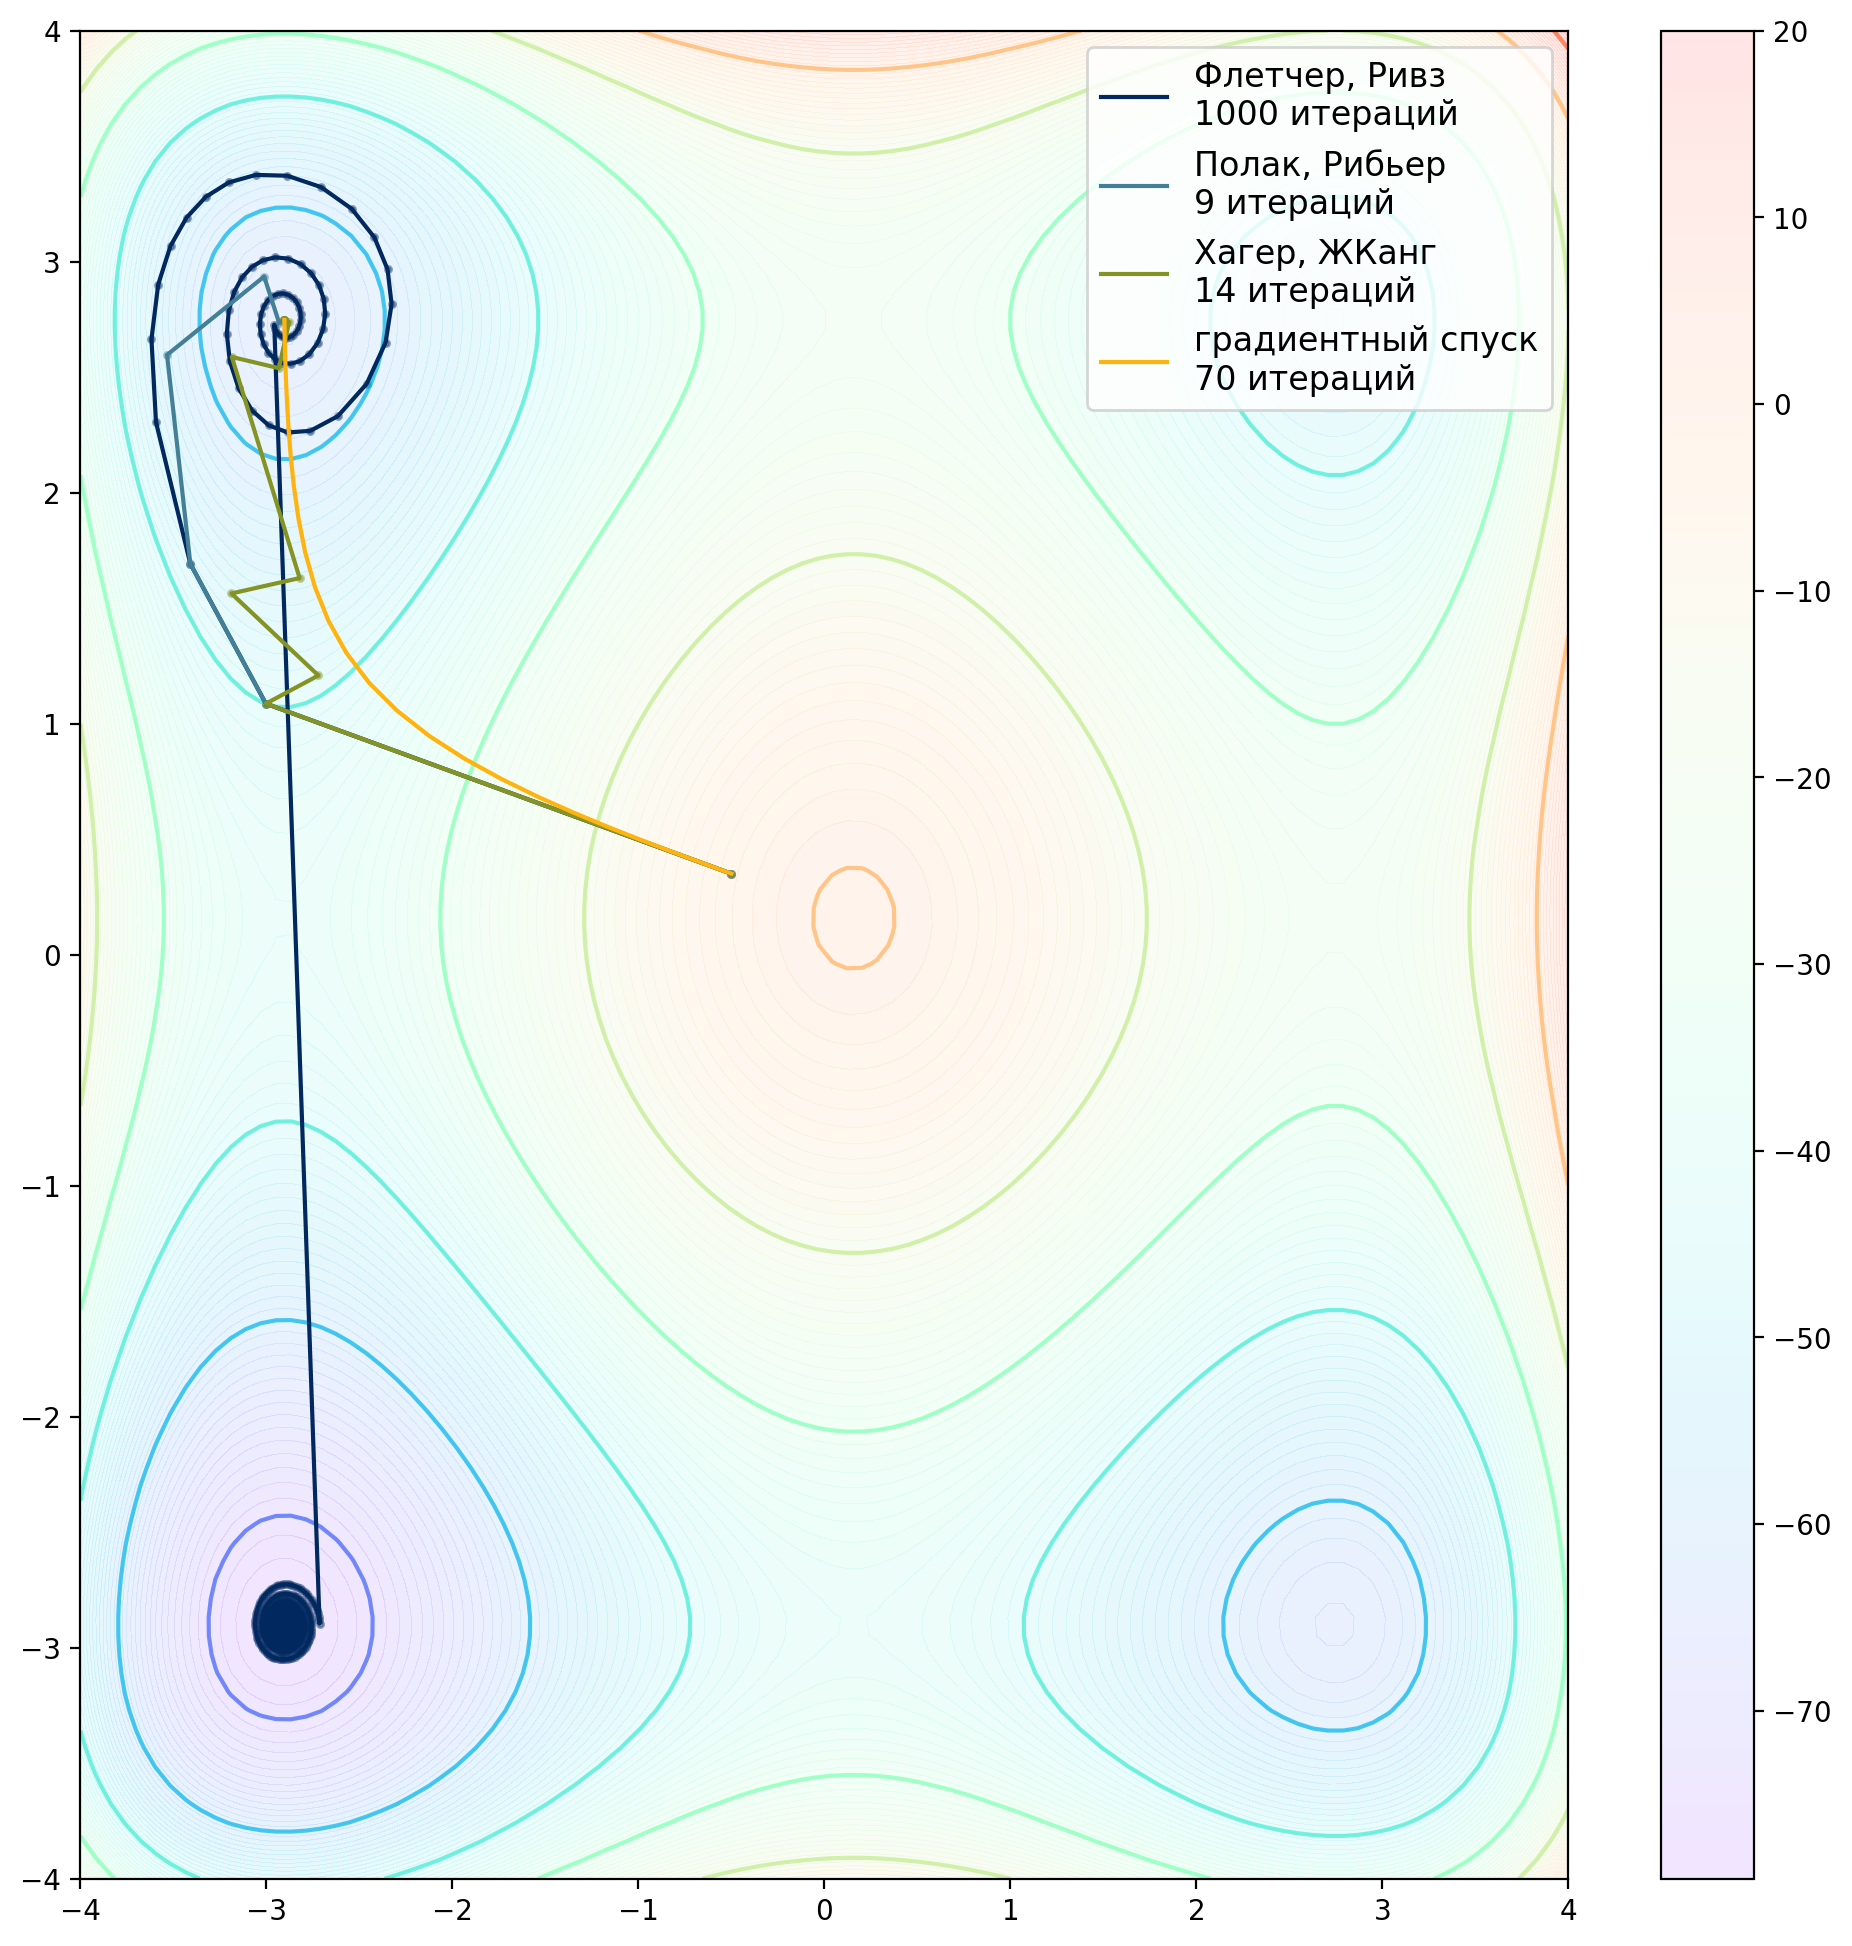
\includegraphics[width=0.7\textwidth]{grad_2.png}    
    \end{center}
\end{frame}


\begin{frame}
    \frametitle{Метод сопряженных градиентов}
    \begin{center}
        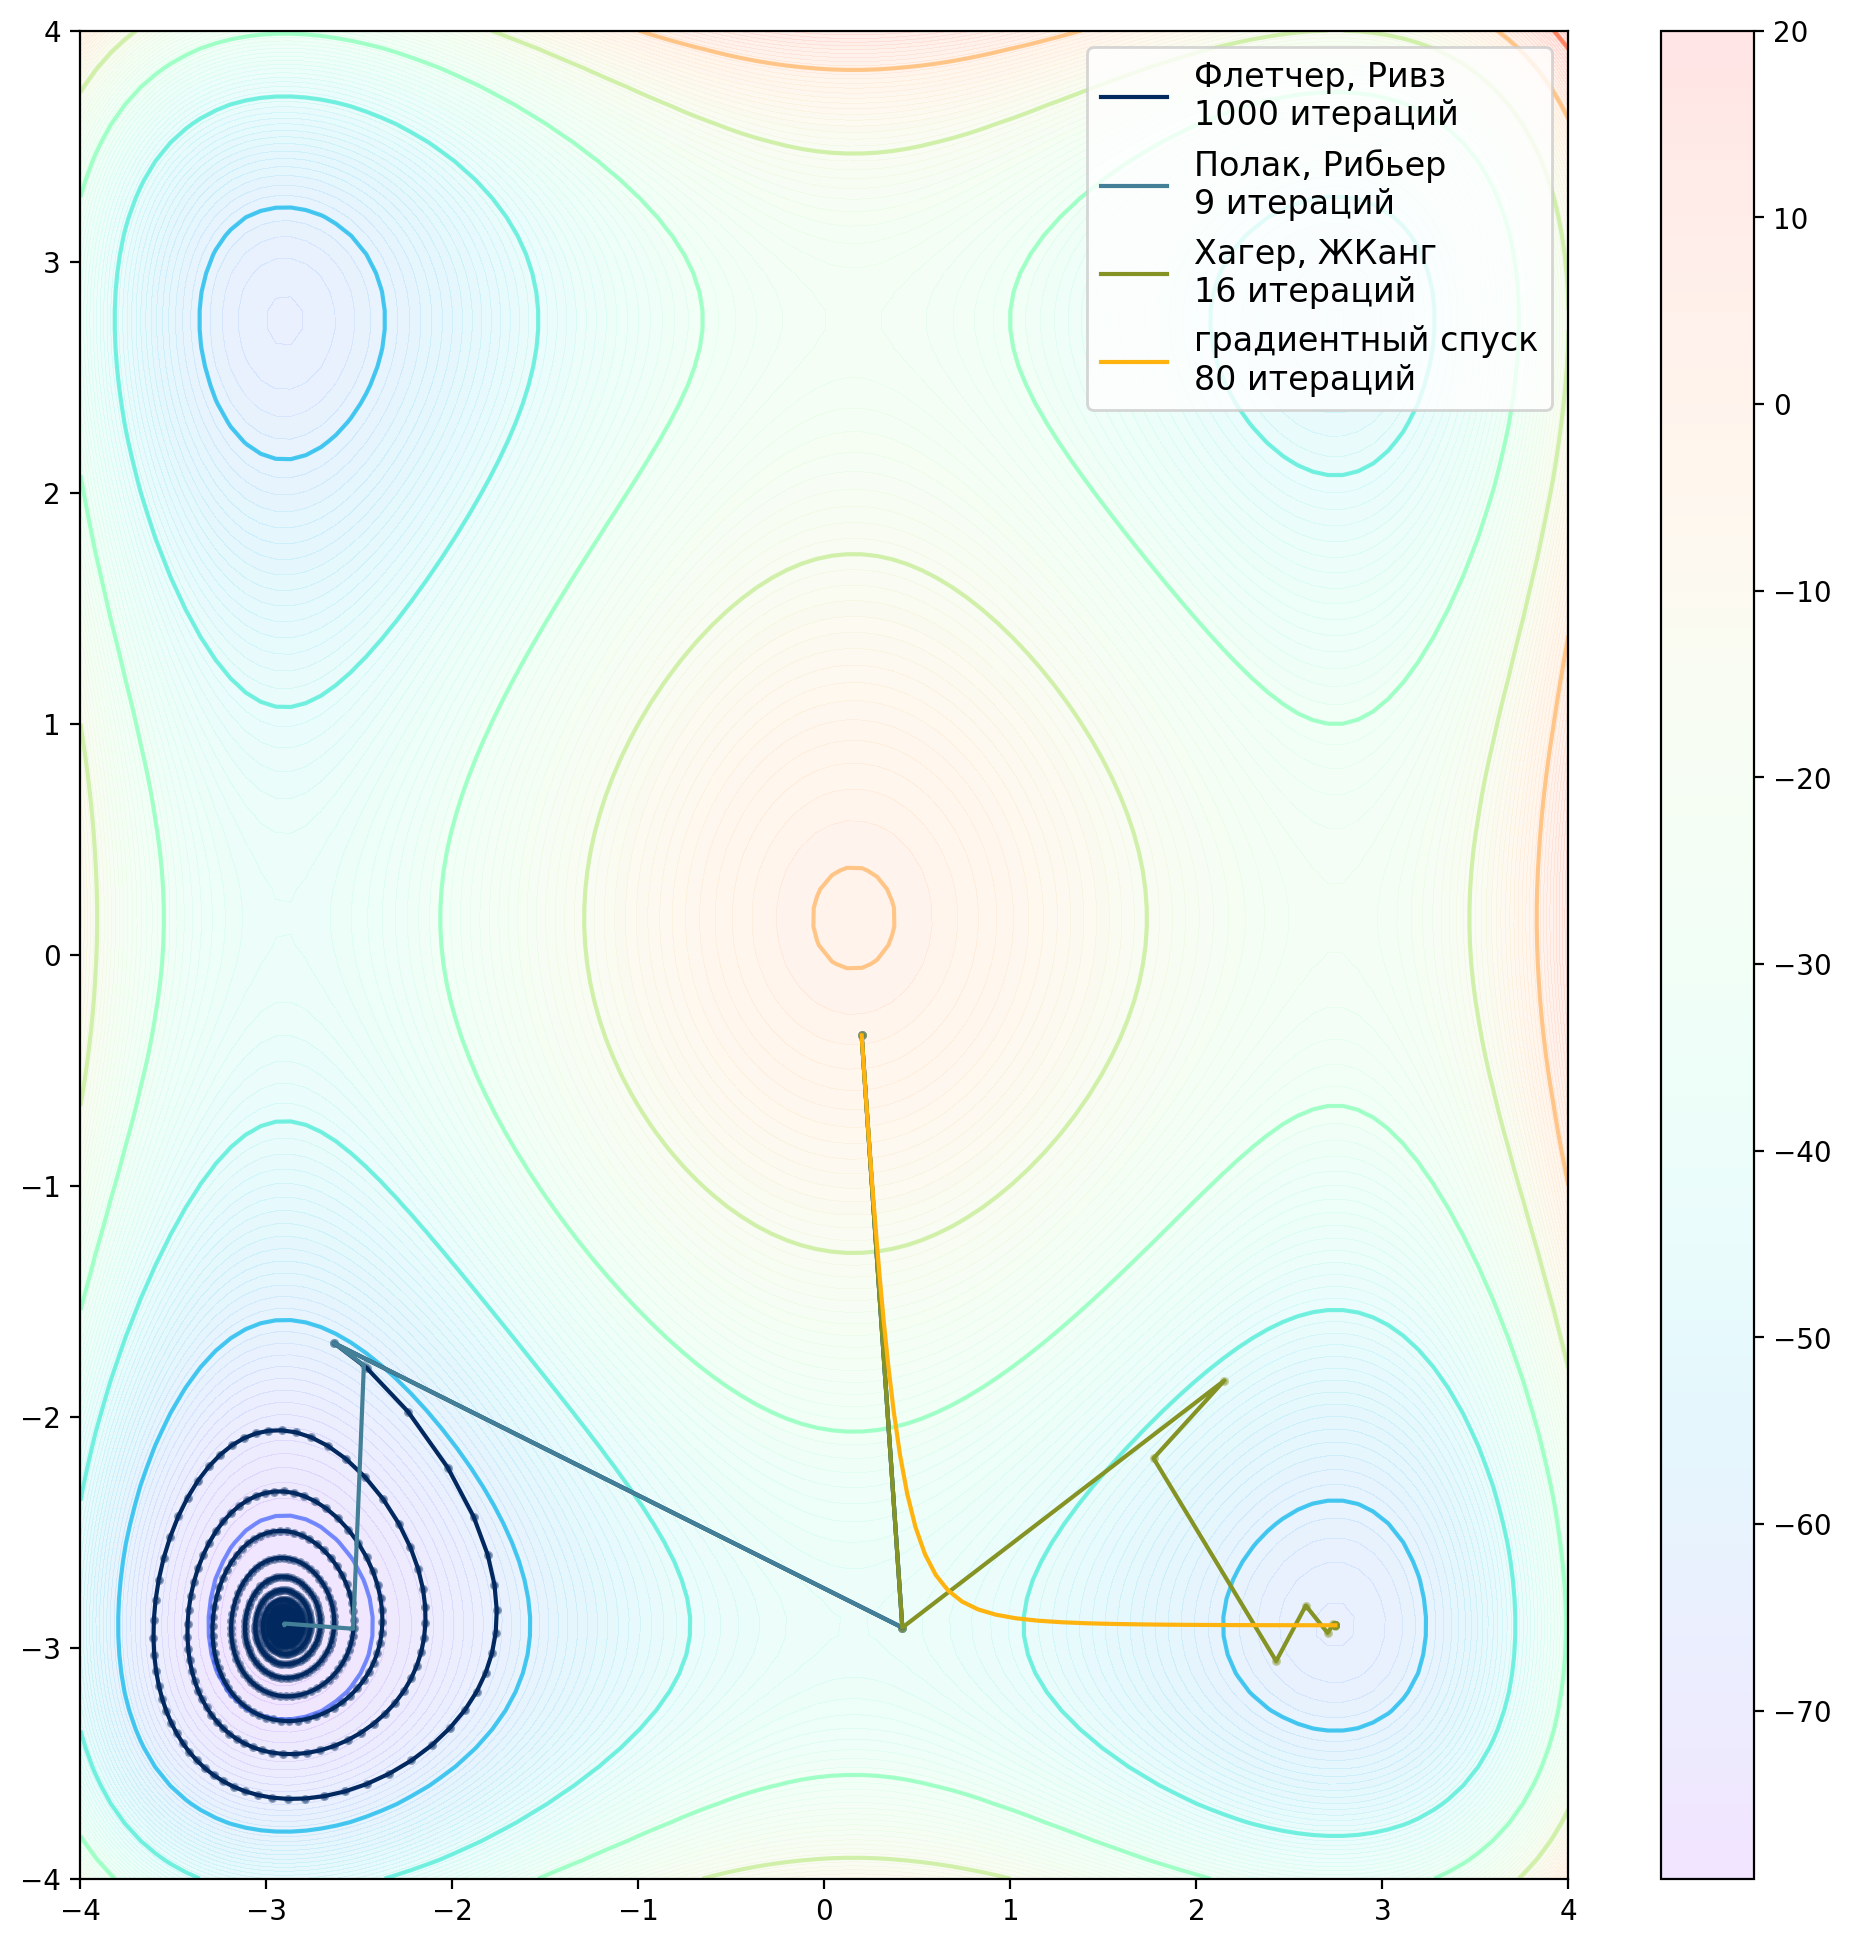
\includegraphics[width=0.7\textwidth]{grad_3.png}    
    \end{center}
\end{frame}

\begin{frame}
    \frametitle{Стохастический градиентный спуск}
    \begin{columns}
        \column{0.5\textwidth}
        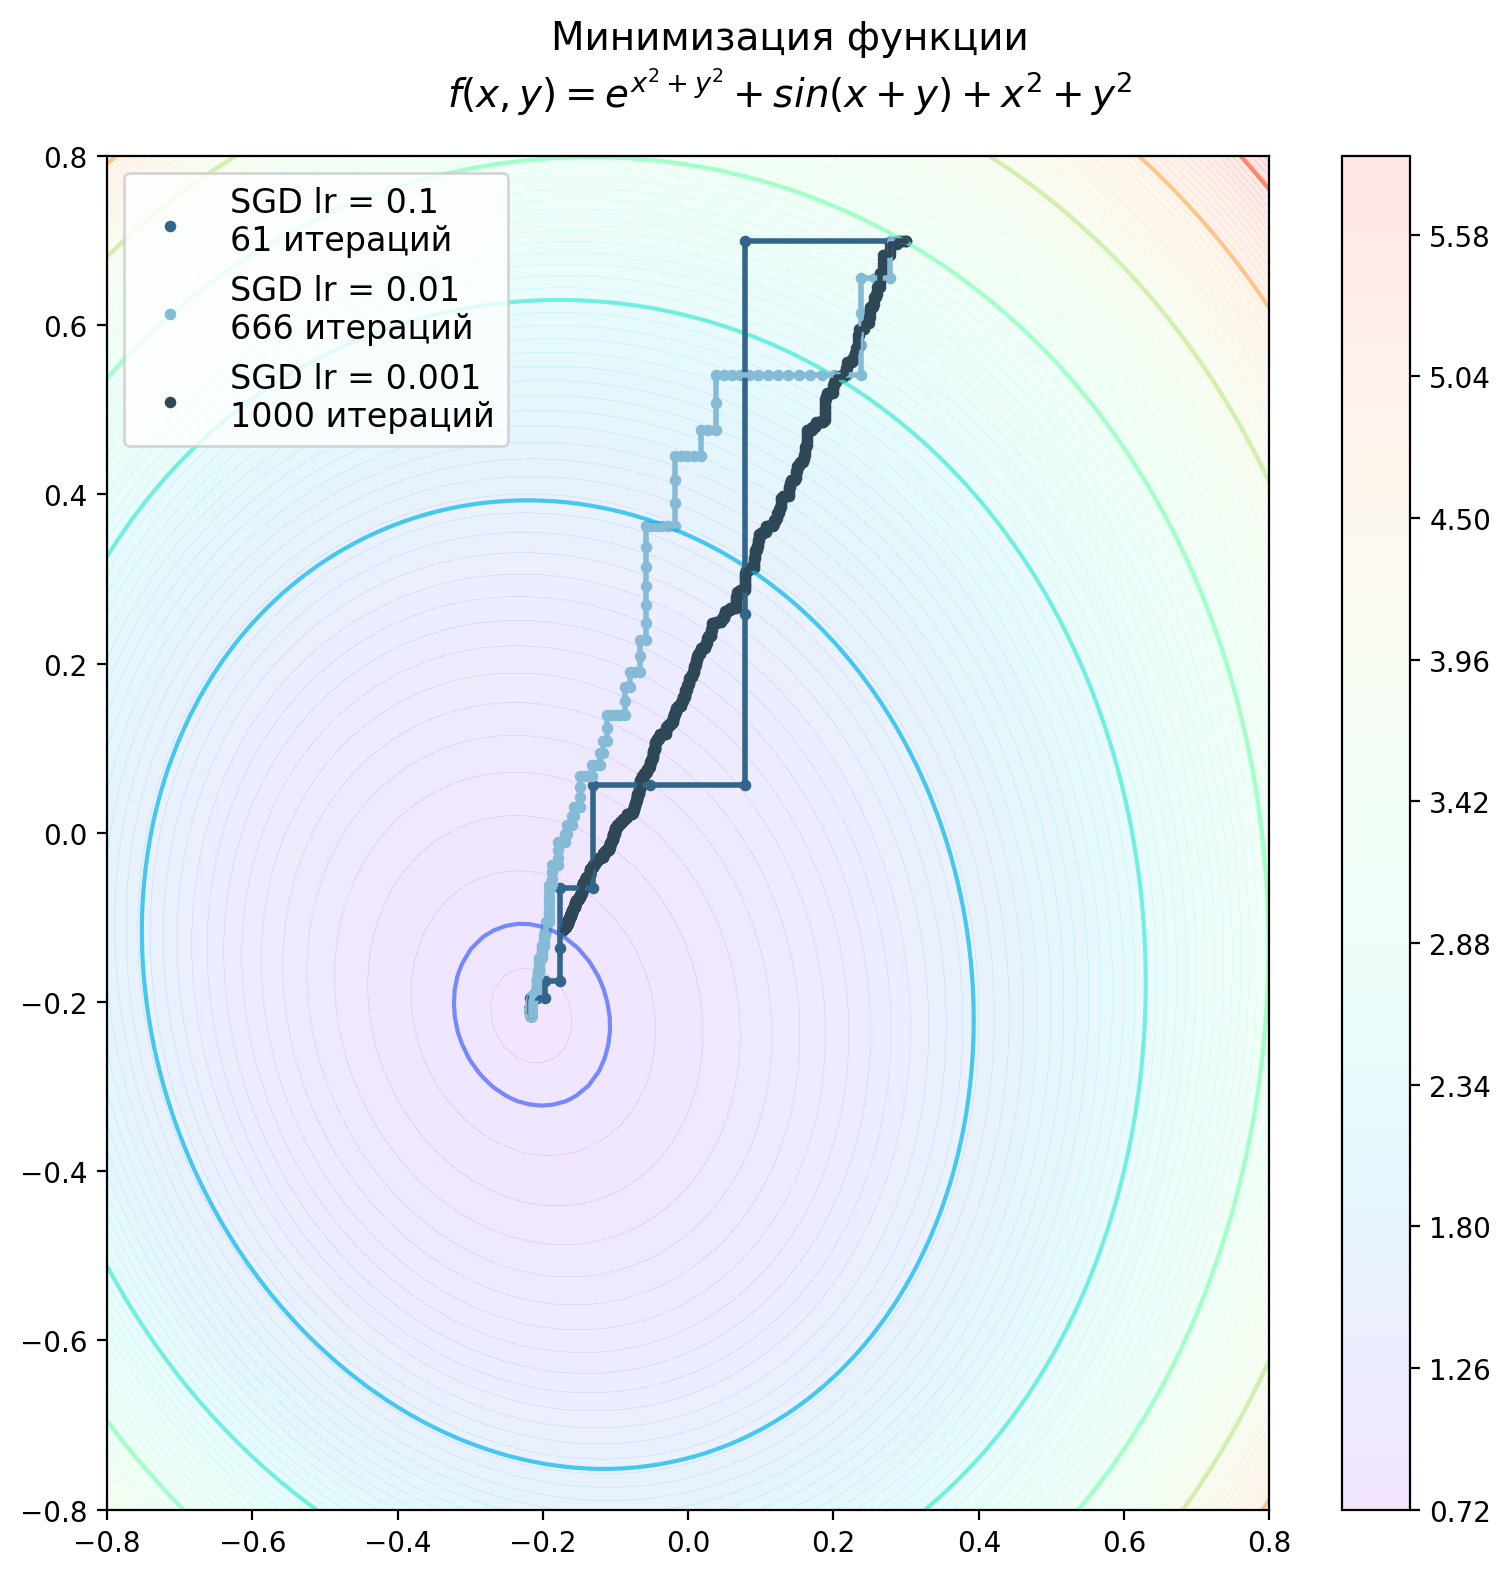
\includegraphics[width = 1\textwidth]{stochastic_gd.png}
        \column{0.5\textwidth}
    \begin{center}
        \begin{itemize}
            \item Выбрать начальную точку $x_0 \in R^{N}$, величину шага $\alpha$, число $b \leq N$.
            \item Пока не выполнено условие остановки
            \begin{enumerate}
                \item Случайно выбираем $N$ попарно различных индексов: $\{n_i\}_{i = 1}^{b}$, $n_i < N$
                \item Составим вектор $d = (0, \dots, \frac{\partial f}{\partial x_{n_{1}}}, \dots, \frac{\partial f}{\partial x_{n_{b}}}, 0, 0, \dots) \in R^{N}$
                \item Шаг стохастического градиентного спуска 
            \end{enumerate}
        \end{itemize}
        \begin{fequation}
            x_{k+1} = x_{k} - \alpha d
        \end{fequation}
    \end{center}
    \end{columns}
\end{frame}


\begin{frame}
    \frametitle{Стохастический градиентный спуск}
    \begin{center}
        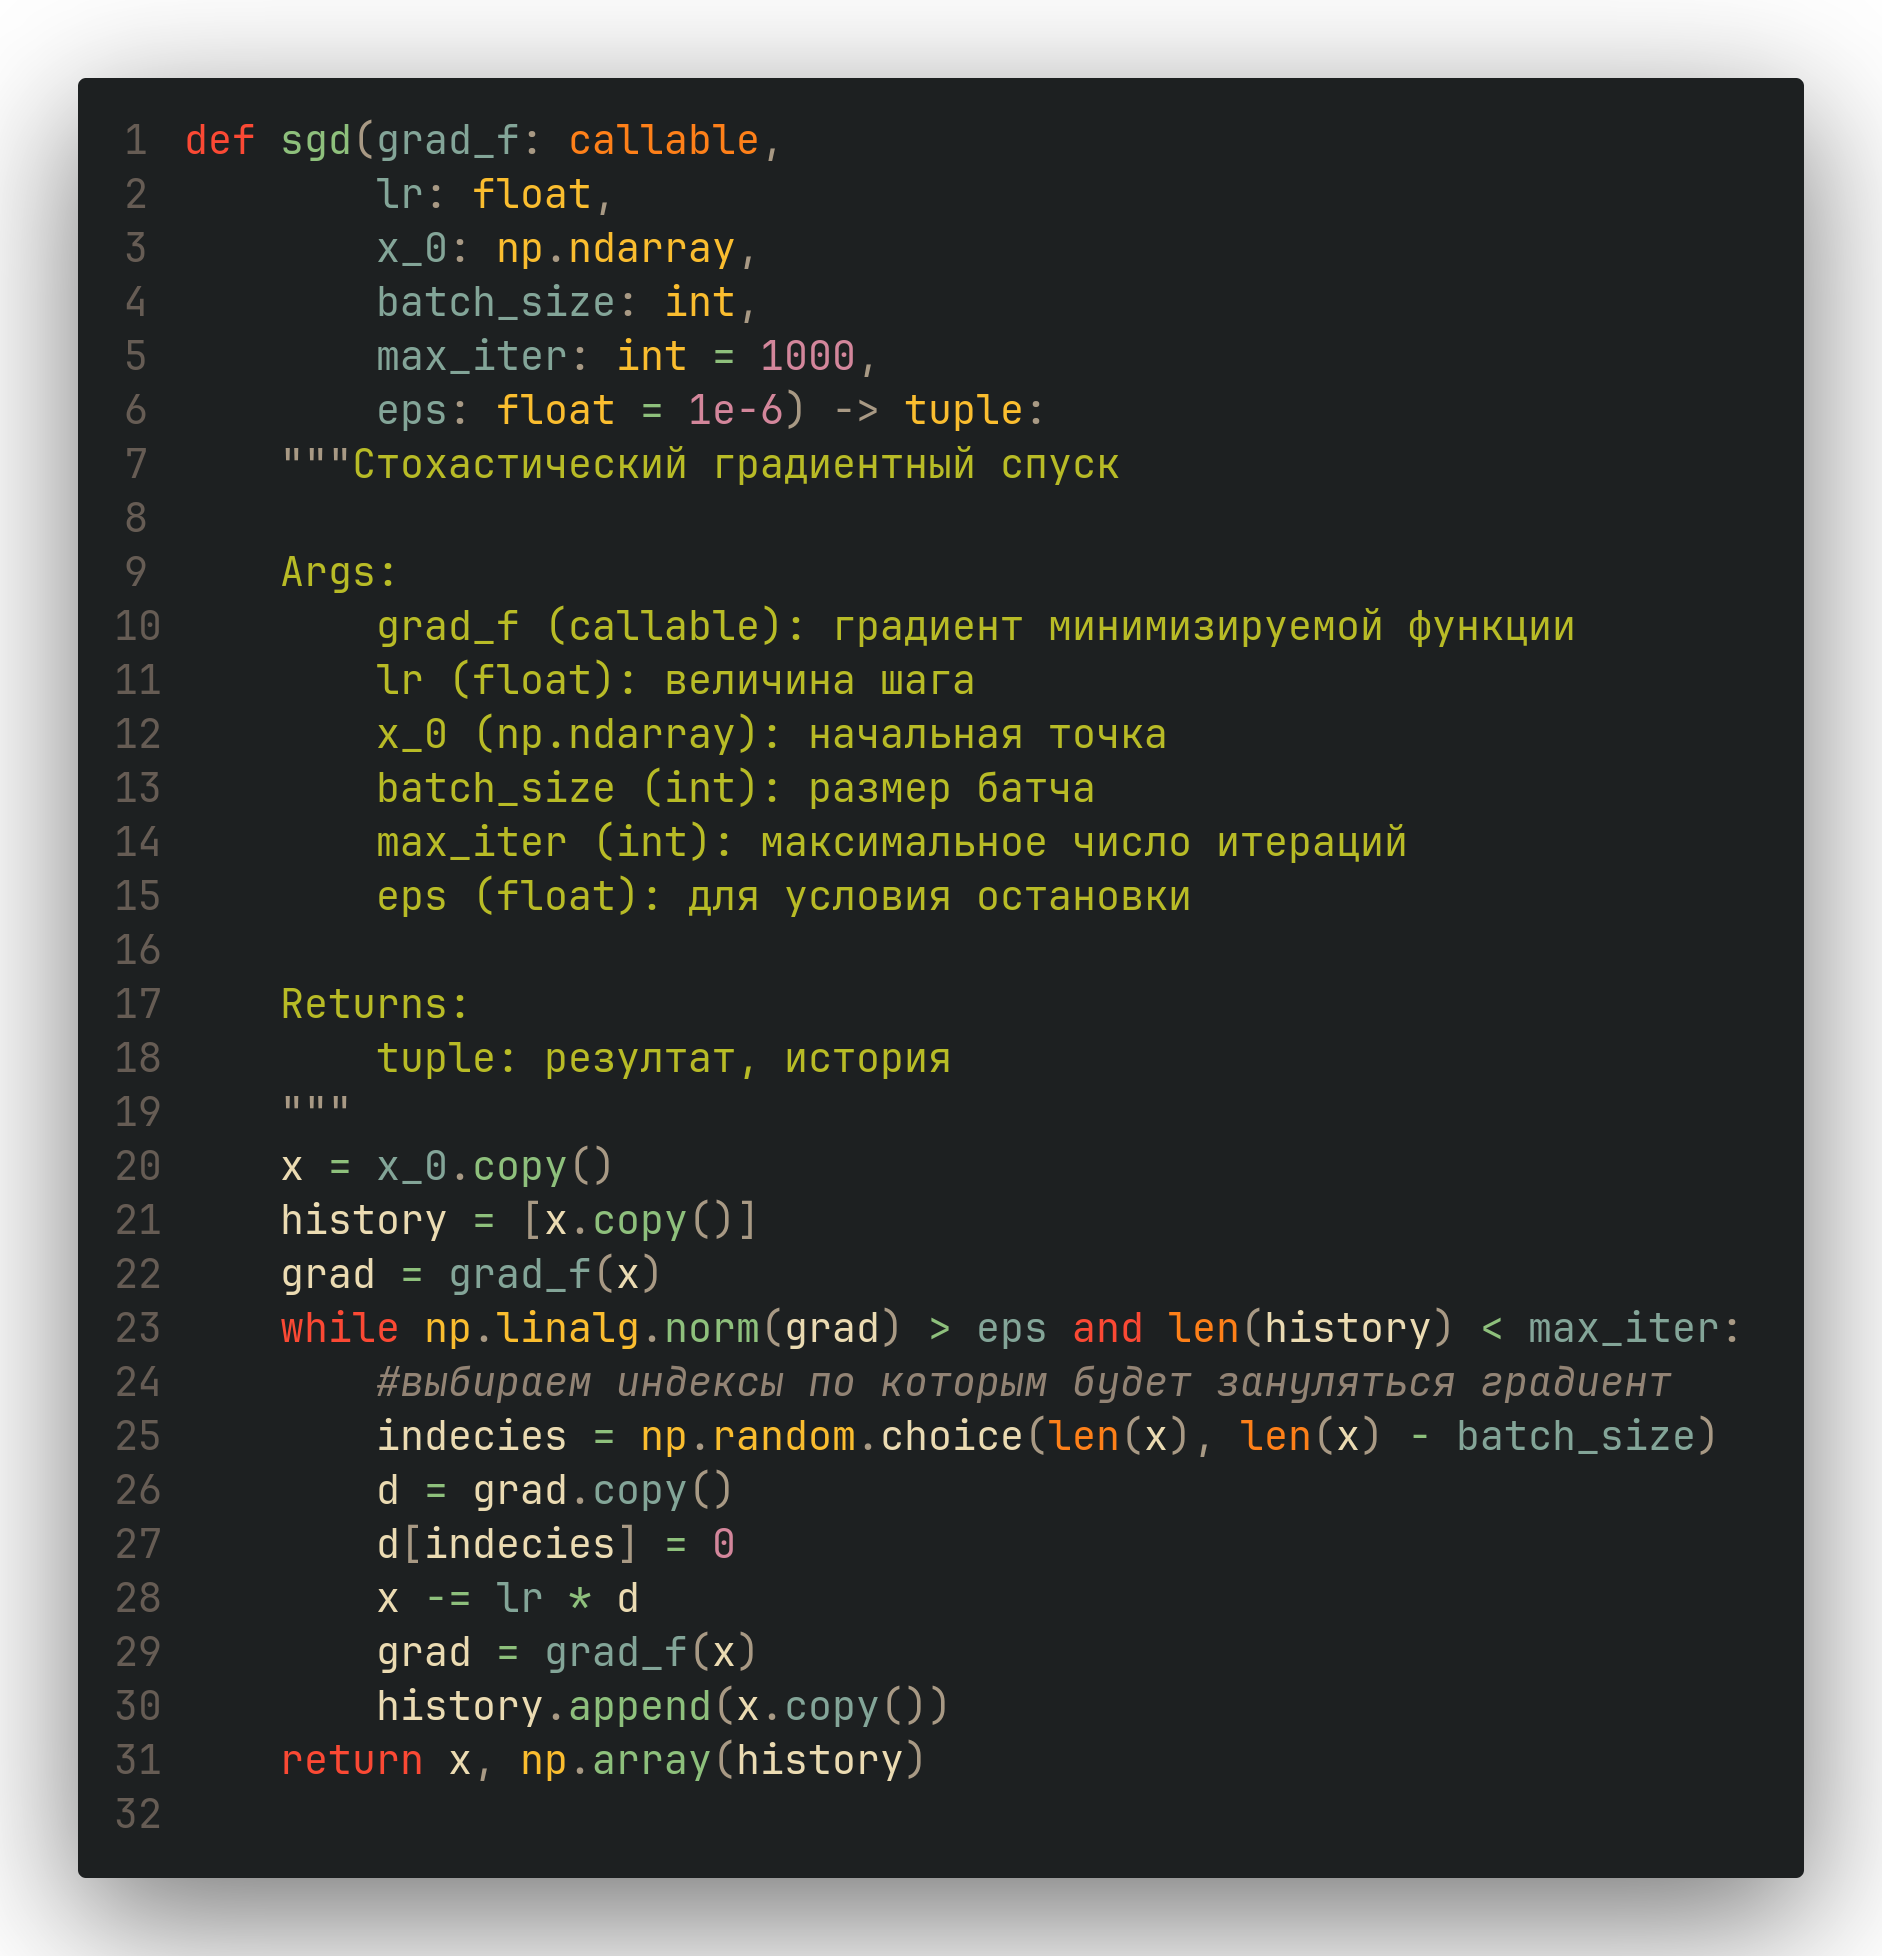
\includegraphics[width=0.7\textwidth]{code_stochastic.png}    
    \end{center}
\end{frame}

\begin{frame}
    \frametitle{Momentum}
    \begin{columns}
        
    \column{0.5\textwidth}
    \begin{center}
        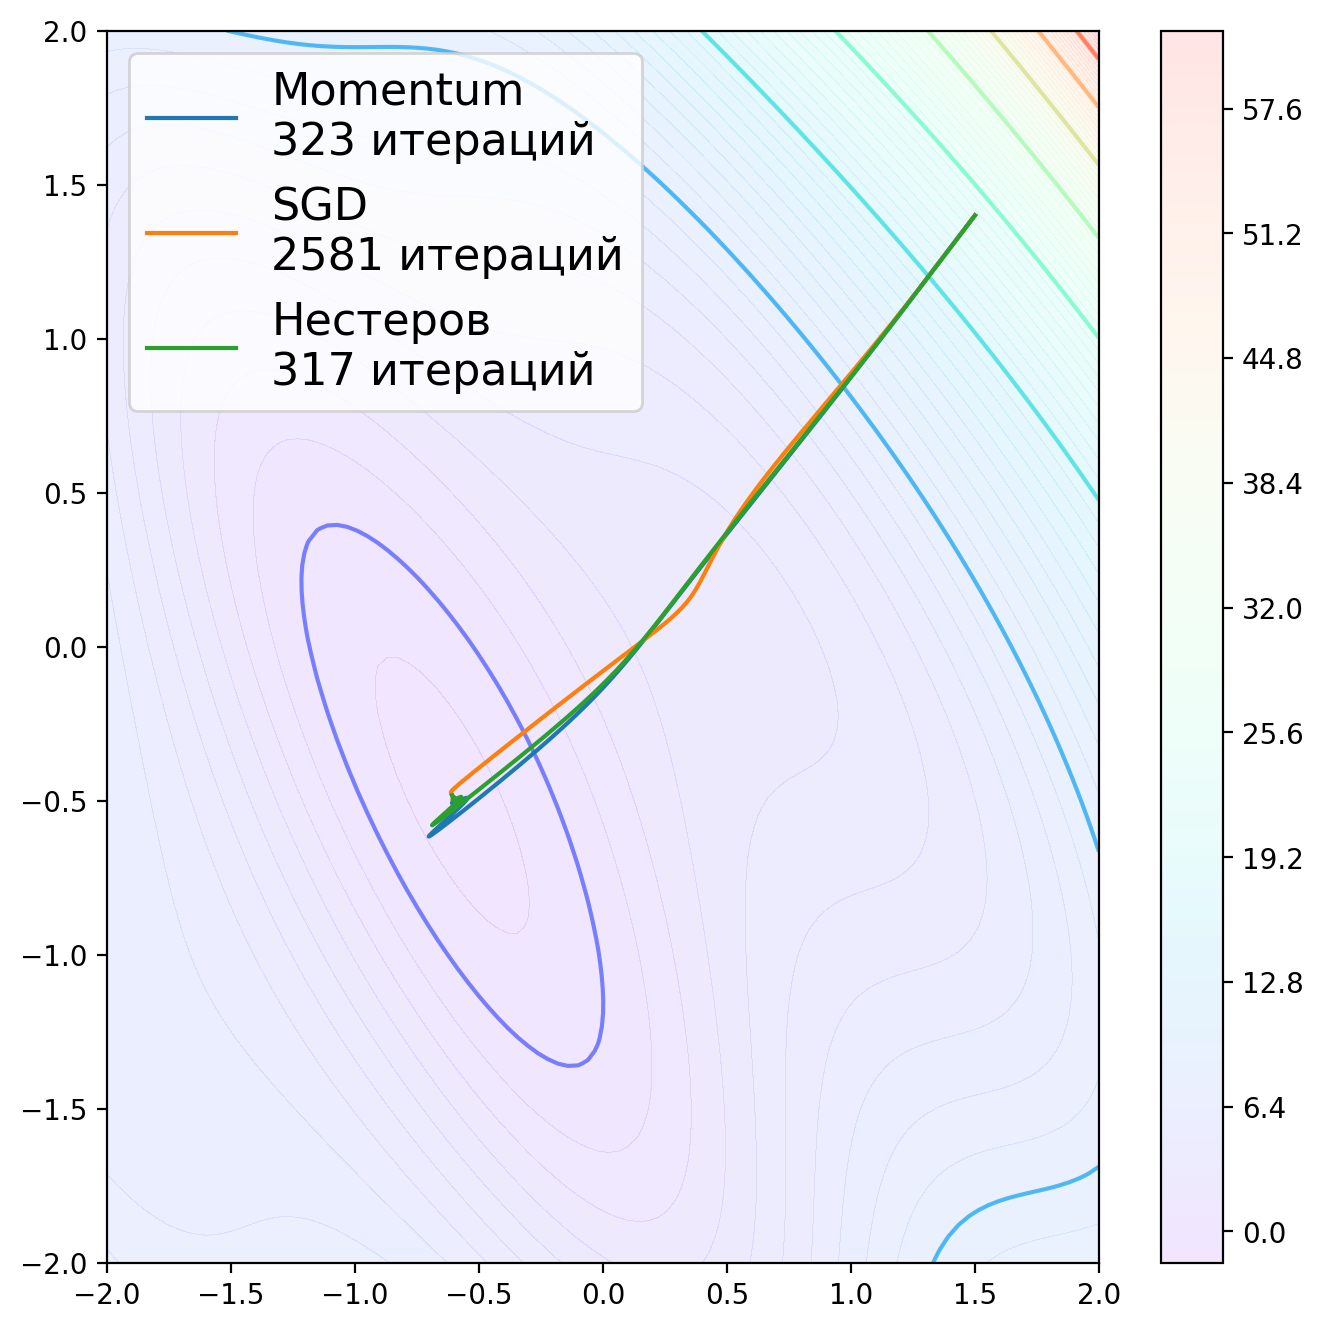
\includegraphics[width = 0.9 \textwidth]{momentum.png}
    \end{center}
    \column{0.5 \textwidth}
    Алгоритм momentum - градиентный спуск, учитывающий предыдущее направление.
    \begin{fequation}
        x_{k + 1} = x_{k} - \alpha \nabla f(x_k) + \beta (x_{k} - x_{k - 1})
    \end{fequation}
    Формулировка Нестерова
    \begin{fequation}
        x_{k + 1} = x_{k} - \alpha (\nabla f(x_k) + \beta (x_{k} - x_{k - 1}))
    \end{fequation}
    \end{columns}
\end{frame}

\begin{frame}
    \frametitle{Почему momentum работает?}
    Алгоритм momentum аналогичен алгоритму <<скользящее среднее>>, используемого для фильтрации сигналов.
    Временной ряд градиентов <<сглаживается>>
    \begin{center}
        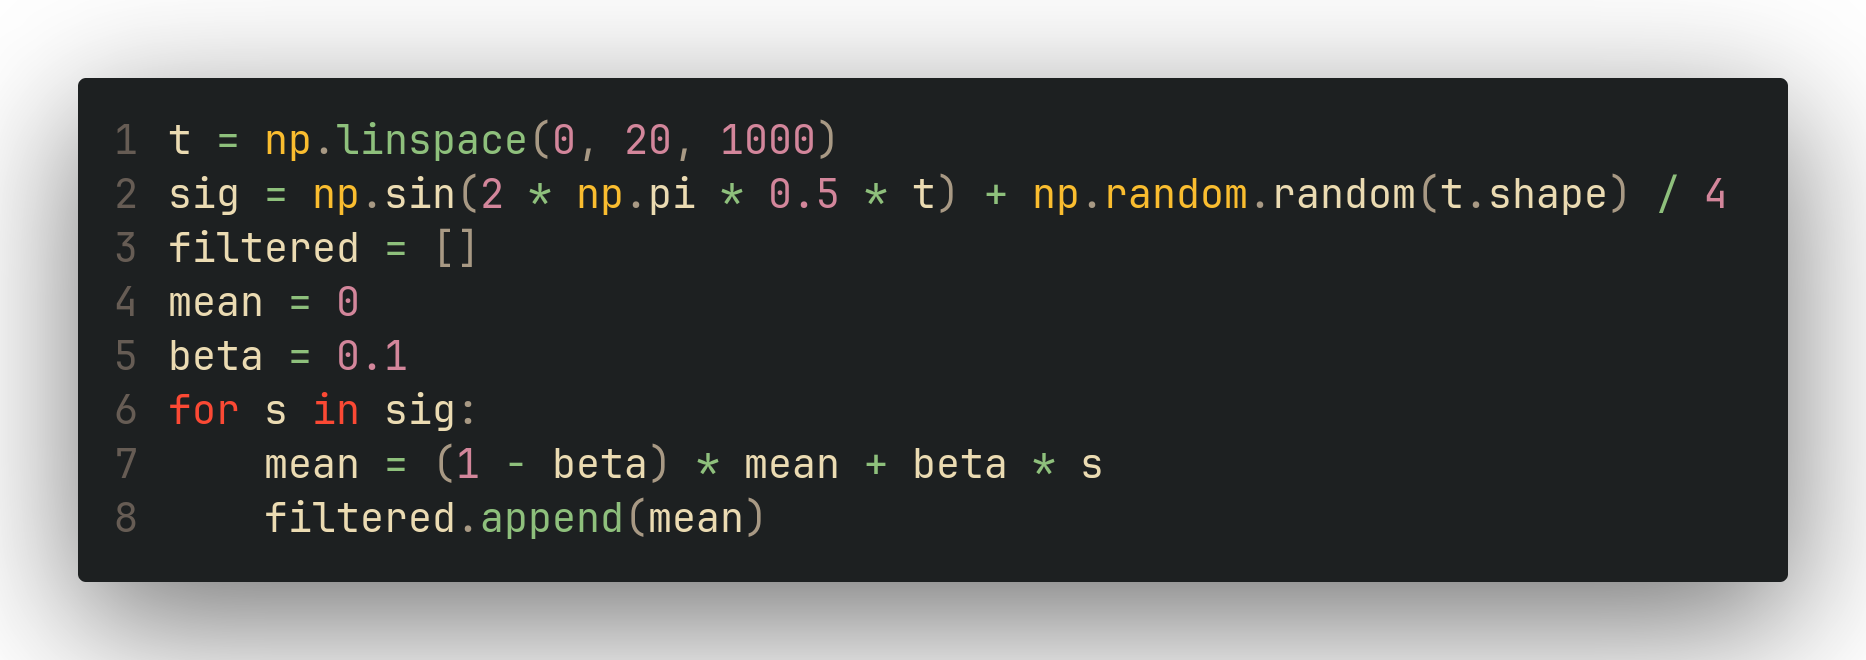
\includegraphics[width = 1\textwidth]{code_smoving_avarage.png}
        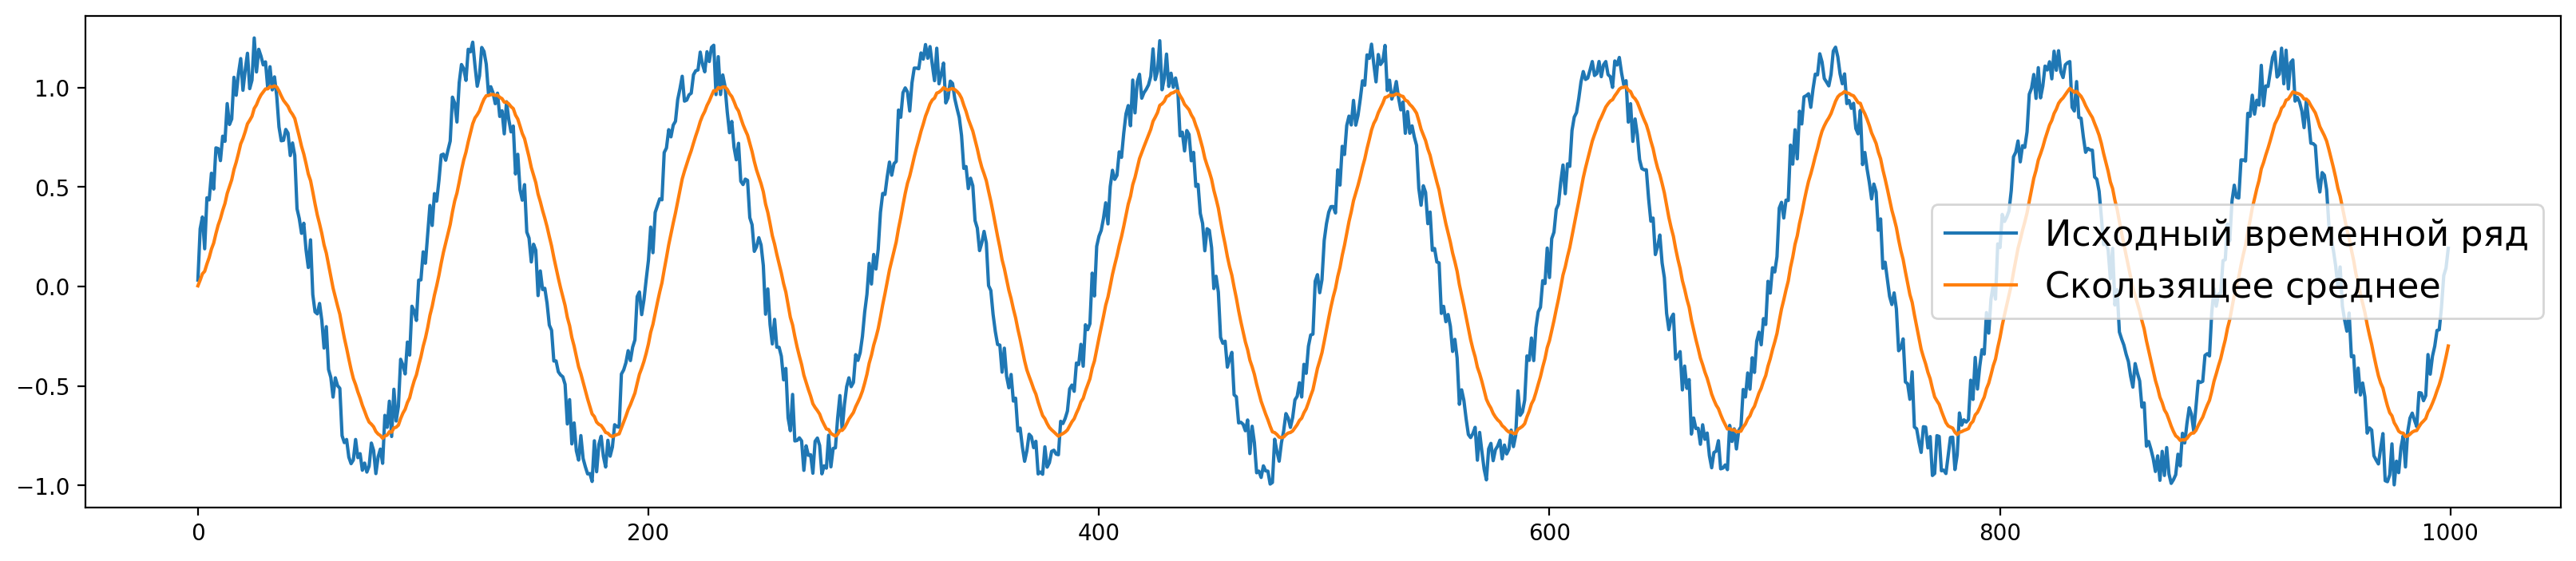
\includegraphics[width = 1 \textwidth]{moving_avarage.png}
    \end{center}
\end{frame}

\begin{frame}
    \frametitle{Адаптивные методы - RMSprop}
    \begin{columns}
    \column{0.5 \textwidth}
    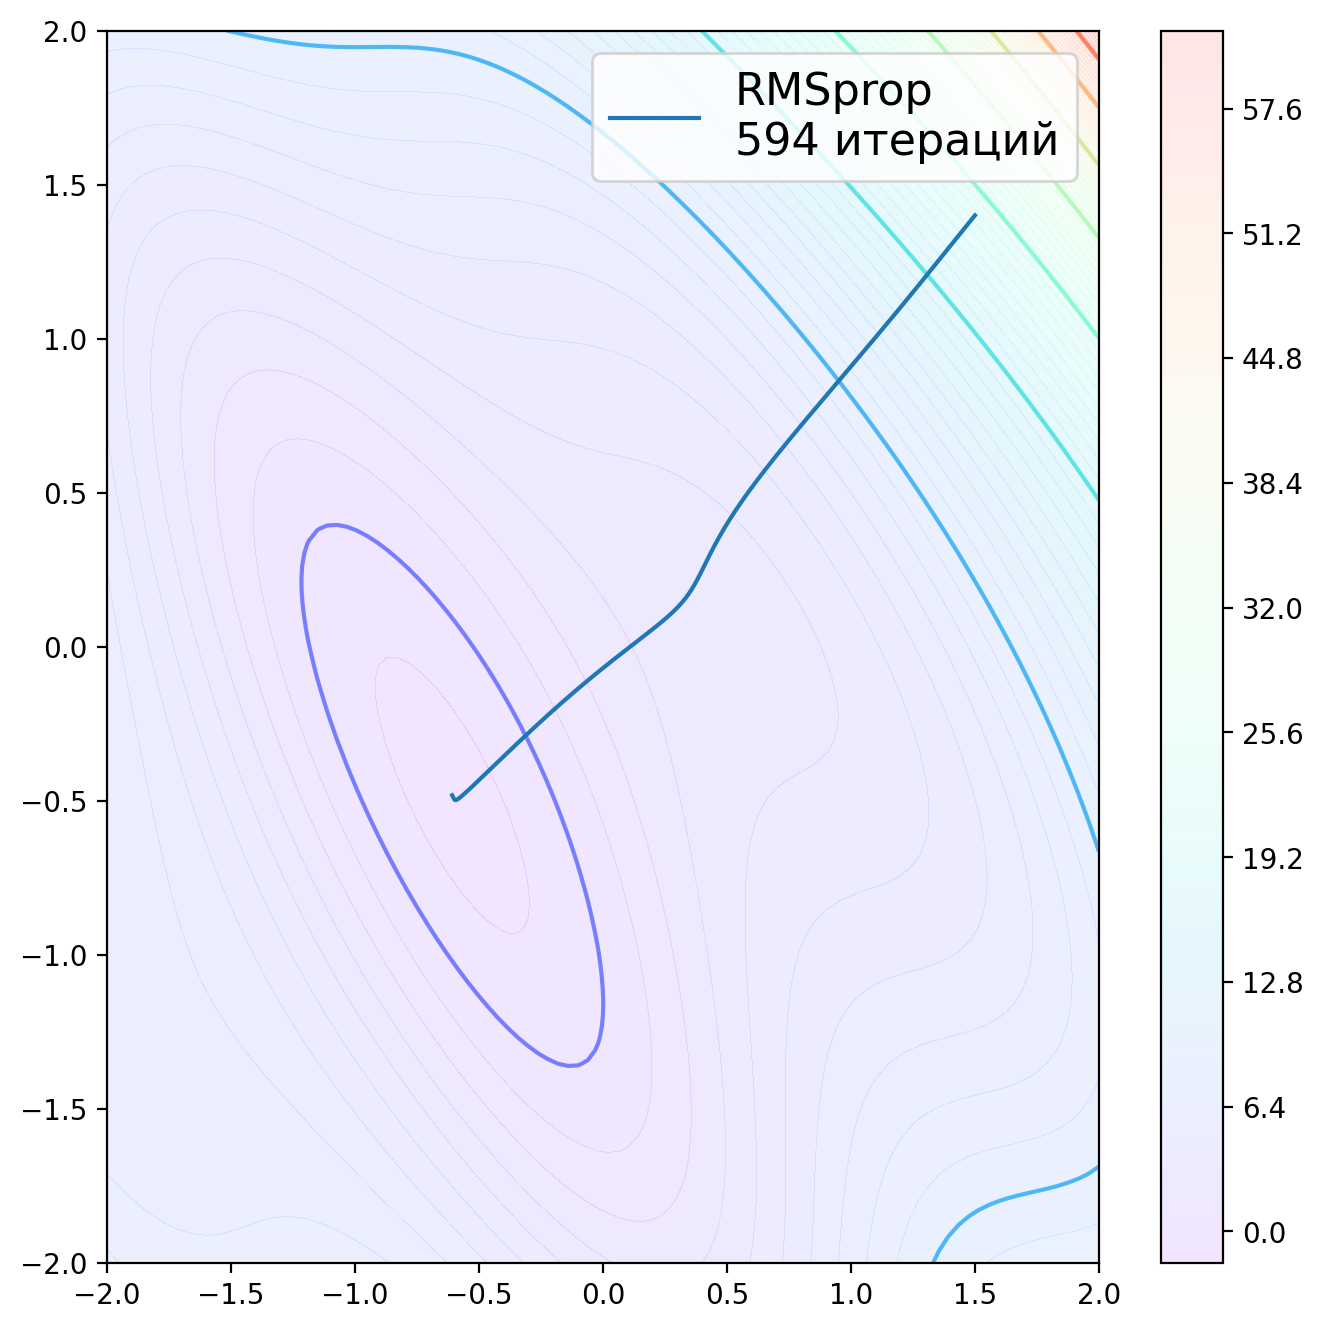
\includegraphics[width = 1\textwidth]{rms.png}
    \column{0.5\textwidth}
    \begin{fequation}
        V_{t + 1} = \alpha V_{t} + (1 - \alpha) \nabla f(x_t)^2 
    \end{fequation}
    \begin{fequation}
    x_{t + 1} = x_{t} - \gamma \frac{\nabla f(x_t)}{\sqrt{V_{t+1}} + \epsilon}
    \end{fequation}
    При вычислении $V$ используем поэлементное возведение в квадрат. При вычислениии $x$ - поэлементное деление и взятие корня.
    \end{columns}
\end{frame}

\begin{frame}
    \frametitle{Адаптивные методы - Adam}
    Скользящее среднее используется не только для оценки величины шага, но и для оценки <<момента>>.
    \begin{columns}
    \column{0.5 \textwidth}
    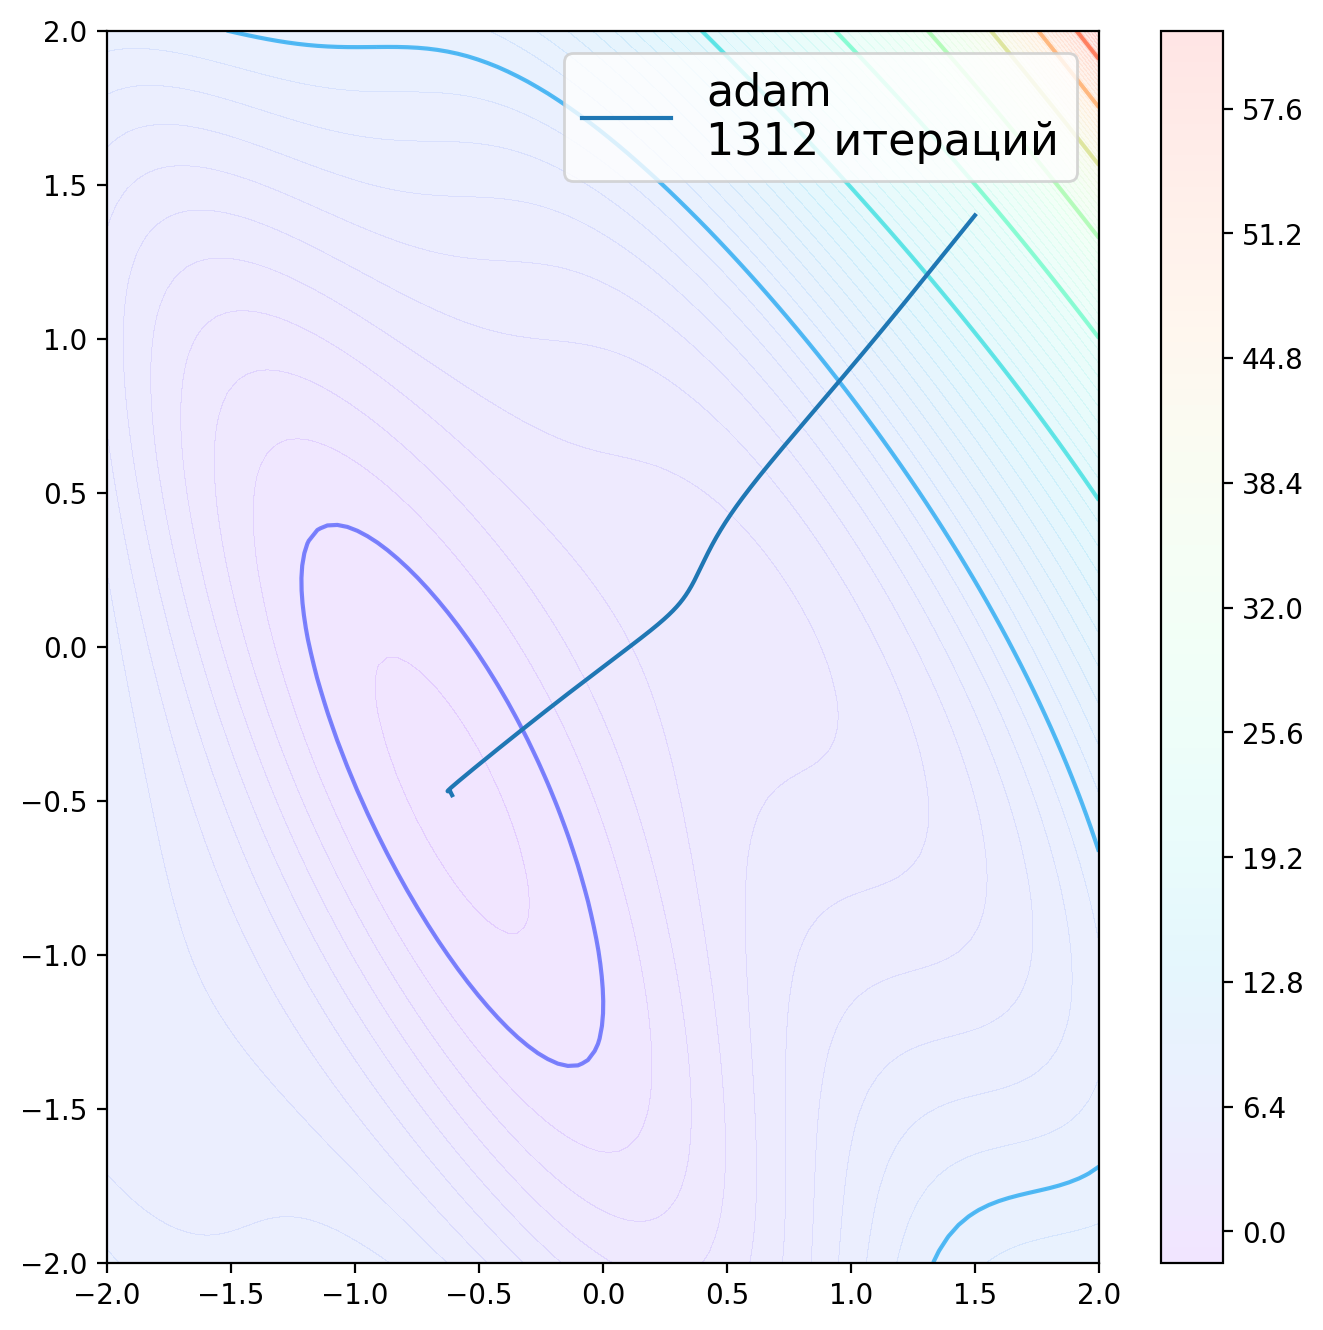
\includegraphics[width = 1\textwidth]{adam.png}
    \column{0.5\textwidth}
    \begin{fequation}
        m_{t + 1} = \beta V_t + (1 - \beta) \nabla f(x_t)
    \end{fequation}
    \begin{fequation}
        V_{t + 1} = \alpha V_{t} + (1 - \alpha) \nabla f(x_t)^2 
    \end{fequation}
    \begin{fequation}
        x_{t+1} = x_{t} - \gamma \frac{m_{t + 1}}{\sqrt{V_{t+1}} + \epsilon}
    \end{fequation}
    
    \end{columns}
\end{frame}

\begin{frame}
    \begin{center}
        \huge{Спасибо за внимание!}       
    \end{center}
 
\end{frame}

\end{document}
